% =================================================================================================
% File:			content_files.tex
% Description:	Defiinisce i capitoli presenti nel documento
% Created:		2015-02-23
% Author:		Tesser Paolo
% Email:		tesser.paolo@mashup-unipd.it
% =================================================================================================
% Modification History:
% Version		Modifier Date		Change											Author
% 0.0.1 		2015-02-23 			sistemato header								Tesser Paolo
% =================================================================================================
%
% =================================================================================================
%

% DEFINIZIONE DEI CONTENUTI DEL DOCUMENTO

% =================================================================================================
% File:			introduzione.tex
% Description:	Defiinisce la sezione relativa al capitolo introduttivo del documento
% Created:		2015-04-21
% Author:		Tesser Paolo
% Email:		tesser.paolo@mashup-unipd.it
% =================================================================================================
% Modification History:
% Version		Modifier Date		Change											Author
% 0.0.1 		2015-04-21 			creato scheletro doc e primo abbozzo			Tesser Paolo
% =================================================================================================
%

% CONTENUTO DEL CAPITOLO

\section{Introduzione} % (fold)
\label{sec:introduzione}
	\subsection{Scopo del documento} % (fold)
	\label{sub:scopo_del_documento}
	Questo documento ha come scopo quello di illustrare le procedure da seguire per svolgere le operazioni previste per l'utente amministratore relative al prodotto \projectName. All'utilizzatore non è chiesta nessuna particolare conoscenza informatica. Alcune operazioni richiedono però che esso abbia dimestichezza con i social network e con le possibilità che offrono.
	% subsection scopo_del_documento (end)

	\subsection{Scopo del prodotto} % (fold)
	\label{sub:scopo_del_prodotto}
	\productScope
	% subsection scopo_del_prodotto (end)

	\subsection{Prerequisiti} % (fold)
	\label{sub:prerequisiti}
	TODO (prendere spunto dagli Steakholders)
	% subsection prerequisiti (end)

	\subsection{Problemi e malfunzionamenti} % (fold)
	\label{sub:problemi_e_malfunzionamenti}
	TODO (prendere spunto dagli Steakholders)
	% subsection problemi_e_malfunzionamenti (end)

	\subsection{Glossario} % (fold)
	\label{sub:glossario}
	TODO (forse servirà inserire il glossario in appendice in quanto agli utenti non viene fornito l'altro Glossario) \newline
	\glossarioDesc
	% subsection glossario (end)

	\subsection{Riferimenti} % (fold)
	\label{sub:riferimenti}
		\subsubsection{Normativi} % (fold)
		\label{ssub:normativi}
			\begin{itemize}
				\item \textbf{Analisi dei Requisiti}: \docNameVersionAdR
				\item \textbf{Specifica Tecnica}: \docNameVersionST
			\end{itemize}
		% subsubsection normativi (end)

		\subsubsection{Informativi} % (fold)
		\label{ssub:informativi}
			\begin{itemize}
				\item \textbf{TODO}: TODO;
			\end{itemize}
		% subsubsection informativi (end)
	% subsection riferimenti (end)
% section introduzione (end)
% section introduzione (end) \clearpage \newpage
% =================================================================================================
% File:			tecnologie_utilizzate.tex
% Description:	Defiinisce la sezione relativa a ...
% Created:		2015-02-23
% Author:		Tesser Paolo
% Email:		tesser.paolo@mashup-unipd.it
% =================================================================================================
% Modification History:
% Version		Modifier Date		Change											Author
% 0.0.1 		2015-02-23 			sistemato header								Tesser Paolo
% =================================================================================================
% 0.0.2			2015-03-05			iniziata impostazione contenuto e stesura		Tesser Paolo
% =================================================================================================
% 0.0.3			2015-03-09			aggiunta librerie e sistemata formattazione		Tesser Paolo
% =================================================================================================
%

% CONTENUTO DEL CAPITOLO

\section{Tecnologie utilizzate} % (fold)
\label{sec:tecnologie_utilizzate}
In questa sezione verranno descritte le tecnologie su cui si basa lo sviluppo del progetto. Per ognuna di esse, verrà indicato l’ambito di utilizzo della tecnologia ed i vantaggi/svantaggi che ne derivano.

	\subsection{Linguaggi} % (fold)
	\label{sub:linguaggi}
		\subsubsection{CSS} % (fold)
		\label{ssub:css}
		CSS (Cascading Style Sheets) è il linguaggio che verrà utilizzato per la formattazione delle pagine web offerte dal sistema. \newline
		\textbf{Pro}:
			\begin{itemize}
				\item permette una buona separazione dal contenuto della pagina rispetto a come verrà visualizzata. Questo garantisce un maggiore controllo sull'aspetto grafico e una più facile manutenzione.
			\end{itemize}

		% subsubsection css (end)

		\subsubsection{HTML5} % (fold)
		\label{ssub:html}
		HTML5 è il linguaggio di markup che verrà utilizzato per la strutturazione delle pagine web che l'applicazione andrà ad offrire sia per gli utenti che per gli amministratori del sistema. \newline
		\textbf{Pro}:
			\begin{itemize}
				\item permette di definire in maniera semplice la struttura delle pagine web;
				\item permette una maggiore semantica della pagina web, garantendo così una migliore indicizzazione da parte dei motori di ricerca;
				\item presenza di una vasta documentazione a supporto per i membri del team.
			\end{itemize}
			\noindent
		% subsubsection html (end)

		\subsubsection{Javascript} % (fold)
		\label{ssub:javascript}
		Javascript è il linguaggio di scripting che verrà utilizzato lato client per la creazione e l'interazione con l'interfaccia utente. \newline
		\textbf{Pro}:
			\begin{itemize}
				\item permette alle pagine di essere dinamiche, reagendo a eventi scaturiti dall'utente;
				\item permette di validare in prima istanza i dati inseriti dagli utenti.
			\end{itemize}
		\noindent
		\newline
		\textbf{Contro}:
			\begin{itemize}
				\item il codice è visibile e può essere letto da chiunque.
			\end{itemize}
			\noindent
		% subsubsection javascript (end)

		\subsubsection{JSON} % (fold)
		\label{ssub:json}
		JSON (Javascript Object Notation) è il formato di dati scelto per lo scambio di informazioni tra il client e il server. \newline
		\textbf{Pro}:
			\begin{itemize}
				\item utilizzo semplice tramite Javascript;
				\item formato utilizzato anche dai Google Endpoints che si andranno a sviluppare. (TO DO - da rivedere)
			\end{itemize}
			\noindent
		% subsubsection json (end)

		\subsubsection{Python} % (fold)
		\label{sub:python}
		Python è il linguaggio utilizzato per gestire il back-end dell'applicazione. \newline
		\textbf{Pro}:
			\begin{itemize}
				\item presenza di una code convention molto forte;
				\item permette una potente manipolazione dei dati;
			\end{itemize}
		\noindent
		\newline
		\textbf{Contro}:
			\begin{itemize}
				\item assenza di costrutti come lo switch;
				\item assenza di tipizzazione statica, sarà compito del programmatore rendere esplicito il tipo delle variabili nel codice seguendo delle norme stabiliti nel \docNameVersionNdP.
			\end{itemize}
			\noindent
		% subsubsection python (end)

		\subsubsection{YAML} % (fold)
		\label{ssub:yaml}
		YAML (YAML Ain't a Markup Language) è il formato di fati per la serializzazione di dati utilizzabile da esseri umani. \newline
		La sua scelta è stata vincolata all'utilizzo della Google App Engine con Python. \newline
		\textbf{Pro}:
			\begin{itemize}
				\item formato di una facile comprensione per un umano.
			\end{itemize}
		\noindent
		% subsubsection yaml (end)

	% subsection linguaggi (end)

	\subsection{Framework} % (fold)
	\label{sub:framework}
		\subsubsection{AngularJS} % (fold)
		\label{ssub:angularjs}
		AngularJS è il framework javascript utilizzato per gestire il lato client dell'applicazione. \newline
		\textbf{Pro}:
			\begin{itemize}
				\item presenza di una vasta comunità a supporto;
				\item design pattern MVC e Dependency Injection già presente all'interno del framework.
			\end{itemize}
		\noindent
		% subsubsection angularjs (end)

		\subsubsection{JINJA2} % (fold)
		\label{ssub:jinja}
		TO DO (da decidere)
		% subsubsection jinja (end)

	% subsection framework (end)

	\subsection{Librerie} % (fold)
	\label{sub:librerie}
		\subsubsection{Chart.js} % (fold)
		\label{ssub:chartsjs}
		Chart.js è la libreria di grafici in javascript utilizzata per la generazione della maggior parte dei grafici che l'utente andrà a vedere. La libreria è reperibile al seguente indirizzo: \url{http://www.chartjs.org/}. \newline
		\textbf{Pro}:
			\begin{itemize}
				\item permette ai grafici di essere responsive;
				\item presenza di implementazioni per il framework AngularJS.
			\end{itemize}
		\noindent
		\newline
		\textbf{Contro}:
			\begin{itemize}
				\item assenza di un map chart, che andrà cercato in un'altra libreria.
			\end{itemize}
			\noindent
		% subsubsection chartsjs (end)
		
		\subsubsection{facebook-sdk} % (fold)
		\label{ssub:facebook_sdk}
		Facebook-sdk è la libreria scelta per effettuare in maniera più semplice e astratta le chiamate alle API di Facebook .La libreria è reperibile al seguente indirizzo: \url{https://facebook-sdk.readthedocs.org/en/latest/}. \newline
		\textbf{Pro}:
			\begin{itemize}
				\item è la libreria maggiormente consigliata dalla comunità di Python.
			\end{itemize}
		\noindent
		\newline
		% subsubsection facebook_sdk (end)

	% subsection librerie (end)

	\subsection{Database} % (fold)
	\label{sub:database}

		\subsubsection{Google Cloud Datastore} % (fold)
		\label{ssub:datastore}
		Google Cloud Datastore è il database NoSQL che viene utilizzato per l'immagazzinamento di tutti i dati. \'E quello fornito dalla Google App Engine. \newline
		\textbf{Pro}:
			\begin{itemize}
				\item permette un forte livello di astrazione che nasconde la complessità dei database schema-less;
				\item presenza di un linguaggio (GQL) utilizzato per l'effettuazione di query con la stessa sintassi di MySQL.
			\end{itemize}
		% subsubsection datastore (end)
	% subsection database (end)


% section tecnologie_utilizzate (end) \clearpage \newpage
% =================================================================================================
% File:			archietettura.tex
% Description:	Defiinisce la sezione relativa a ...
% Created:		2015-02-23
% Author:		Tesser Paolo
% Email:		tesser.paolo@mashup-unipd.it
% =================================================================================================
% Modification History:
% Version		Modifier Date		Change											Author
% 0.0.1 		2015-02-23 			sistemato header								Tesser Paolo
% =================================================================================================
%
% =================================================================================================
%

% CONTENUTO DEL CAPITOLO

\section{Descrizione Architettura} % (fold)
\label{sec:descrizione_architettura}
TO DO
% section descrizione_architettura (end) \clearpage \newpage
% =================================================================================================
% File:			componenti_e_classi.tex
% Description:	Defiinisce la sezione relativa a ...
% Created:		2015-02-23
% Author:		Tesser Paolo
% Email:		tesser.paolo@mashup-unipd.it
% =================================================================================================
% Modification History:
% Version		Modifier Date		Change											Author
% 0.0.1 		2015-02-23 			sistemato header								Tesser Paolo
% =================================================================================================
%
% =================================================================================================
%

% CONTENUTO DEL CAPITOLO

\section{Componenti e Classi} % (fold)
\label{sec:componenti_e_classi}
TO DO
% section componenti_e_classi (end) \clearpage \newpage
% =================================================================================================
% File:			schema_database.tex
% Description:	Defiinisce la sezione relativa a ...
% Created:		2015-02-23
% Author:		Tesser Paolo
% Email:		tesser.paolo@mashup-unipd.it
% =================================================================================================
% Modification History:
% Version		Modifier Date		Change											Author
% 0.0.1 		2015-02-23 			sistemato header								Tesser Paolo
% =================================================================================================
% 0.0.2			2015-03-05			stesura sezione sul db schema-less				Tesser Paolo
% =================================================================================================
%

% CONTENUTO DEL CAPITOLO

\section{Schema Database} % (fold)
\label{sec:schema_database}
Il database utilizzato, sia per quanto riguarda i dati grezzi sia per quanto riguarda i dati aggregati e le varie configurazioni, sarà di tipo schema-less. Questo significa che non c'è un diagramma di come i dati siano in relazione tra loro. \newline
Il modo quindi nel quale saranno salvati, nel database descritto nella sezione \ref{sub:database}, e in che formato viene descritto dal Model dell'applicazione come illustrato alla sezione TO DO. \newline
TO DO (possibili aggiunte)
% section schema_database (end) \clearpage \newpage
% % =================================================================================================
% File:			diagrammi attivita.tex
% Description:	Defiinisce la sezione relativa a ...
% Created:		2015-02-23
% Author:		Tesser Paolo
% Email:		tesser.paolo@mashup-unipd.it
% =================================================================================================
% Modification History:
% Version		Modifier Date		Change											Author
% 0.0.1 		2015-02-23 			sistemato header								Tesser Paolo
% =================================================================================================
% 0.0.2			2015-03-19			cambiata logica diagrammi e estesa				Tesser Paolo
% =================================================================================================
% 0.0.3			2015-03-19			stese le note principali per ogni diagramma		Tesser Paolo
% =================================================================================================
%


% CONTENUTO DEL CAPITOLO

\section{Diagrammi delle attività} % (fold)
\label{sec:diagrammi_delle_attivita}
In questa sezione vengono illustrati i diagrammi delle attività che descrivono le interazione dei diversi tipi di utente con il prodotto. Per ogni utente che interagisce con il sistema verrà rappresentato un diagramma principale delle attività che può svolgere, andando poi a raffinare le singole con ulteriori grafici maggiormente dettagliati. \newline
I diagrammi vengono classificati con il seguente formalismo:
	\begin{center}
		D[Codice]
	\end{center}
	\noindent
Dove [Codice] è un valore gerarchico.

	\subsection{Utente non autenticato} % (fold)
	\label{sub:utente_non_autenticato}
	In questa sezione vengono illustrate le attività che un utente non registrato o non ancora autenticato al sistema può compiere.
		\subsubsection{D1: Attività principali dell'utente non autenticato} % (fold)
		\label{ssub:attivita_principali_dell_utente_non_autenticato}
		\begin{figure}[!htbp]
			\centering
			\centerline{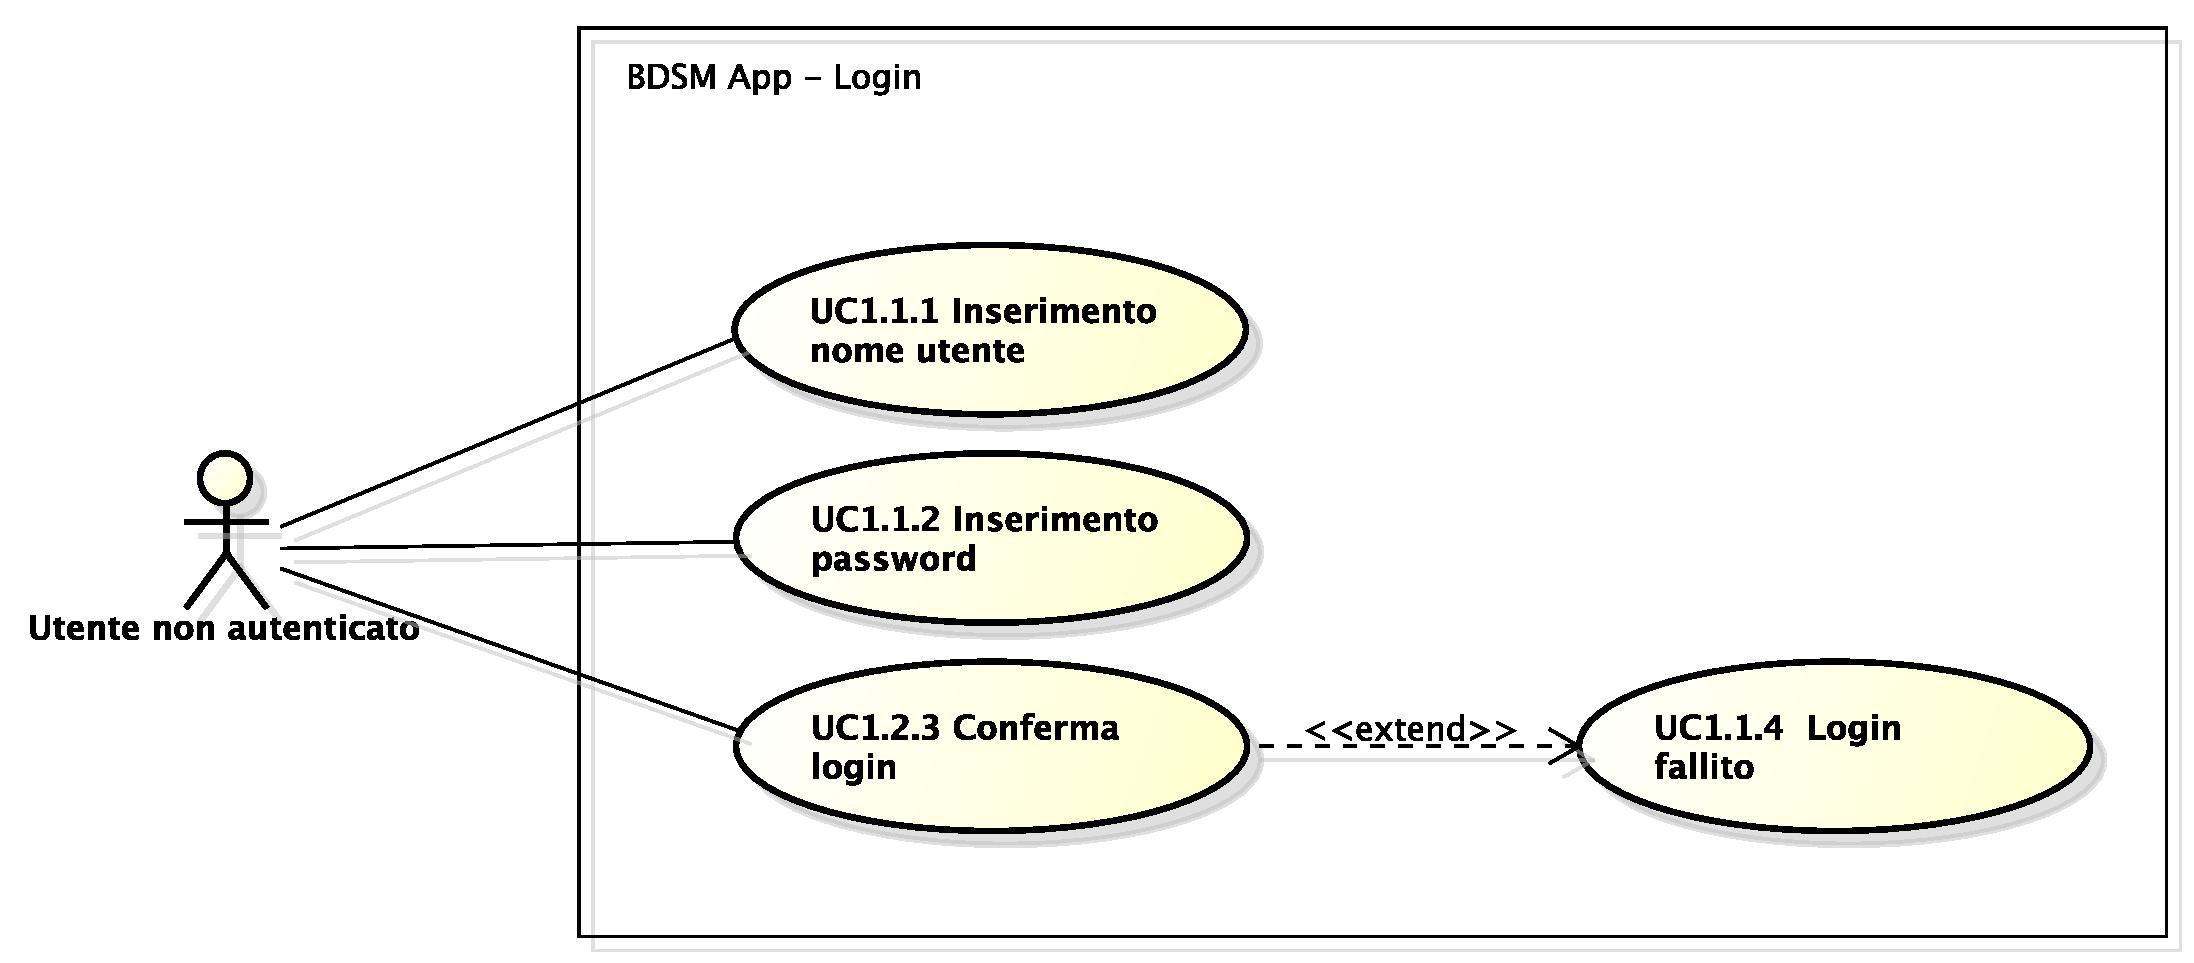
\includegraphics[scale=0.45]{./images/UC1_1.pdf}}
			\caption{D1 - Diagramma delle attività principali dell'utente non autenticato}
		\end{figure}
		[TO DO] (descrizione generale e elenco delle attività principali)

		% subsubsection attività_principali_dell_utente_non_autenticato (end)

		\subsubsection{D1.1: Registrazione al sistema} % (fold)
		\label{ssub:registrazione_al_sistema}
		\begin{figure}[!htbp]
			\centering
			\centerline{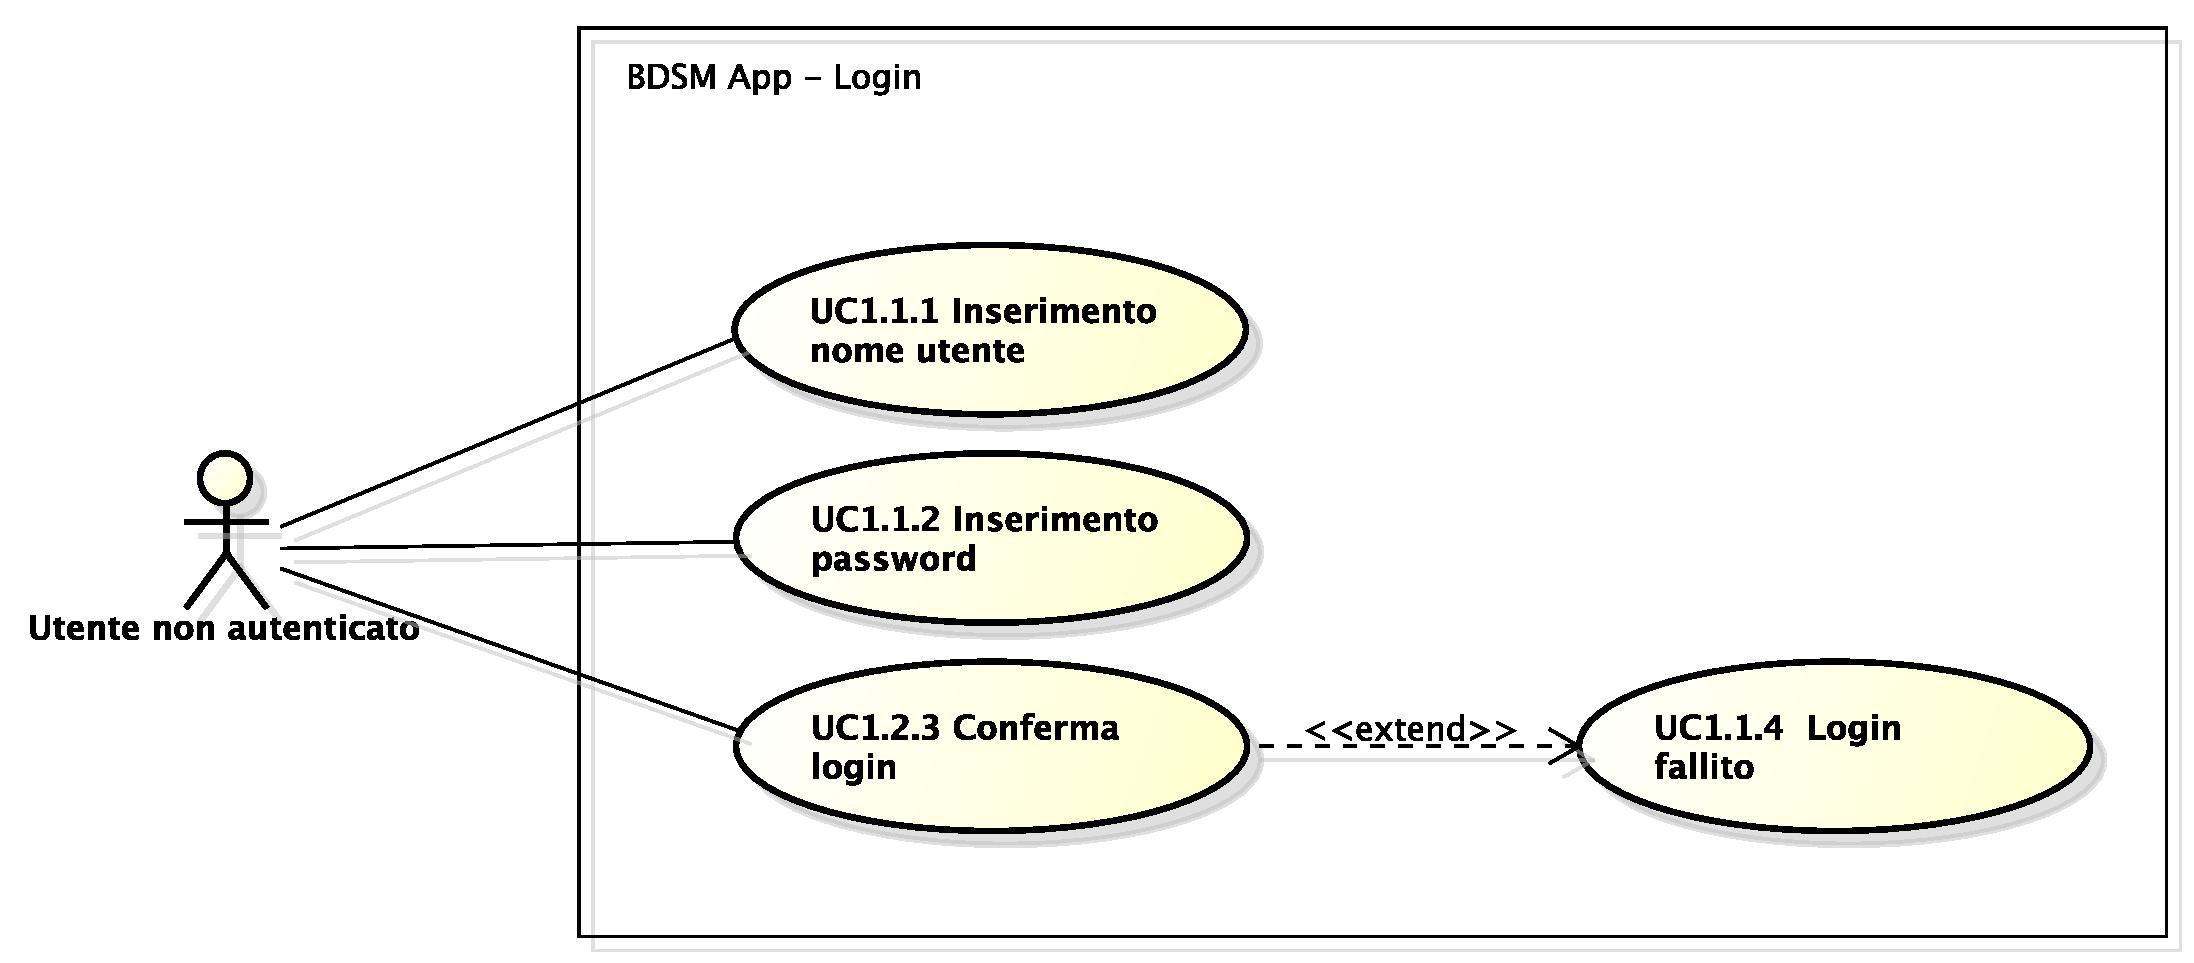
\includegraphics[scale=0.45]{./images/UC1_1.pdf}}
			\caption{D1.1 - Diagramma della registrazione al sistema}
		\end{figure}
		[TO DO] (descrizione generale)
		% subsubsection registrazione_al_sistema (end)

		\subsubsection{D1.2: Accesso al sistema} % (fold)
		\label{ssub:accesso_al_sistema}
		\begin{figure}[!htbp]
			\centering
			\centerline{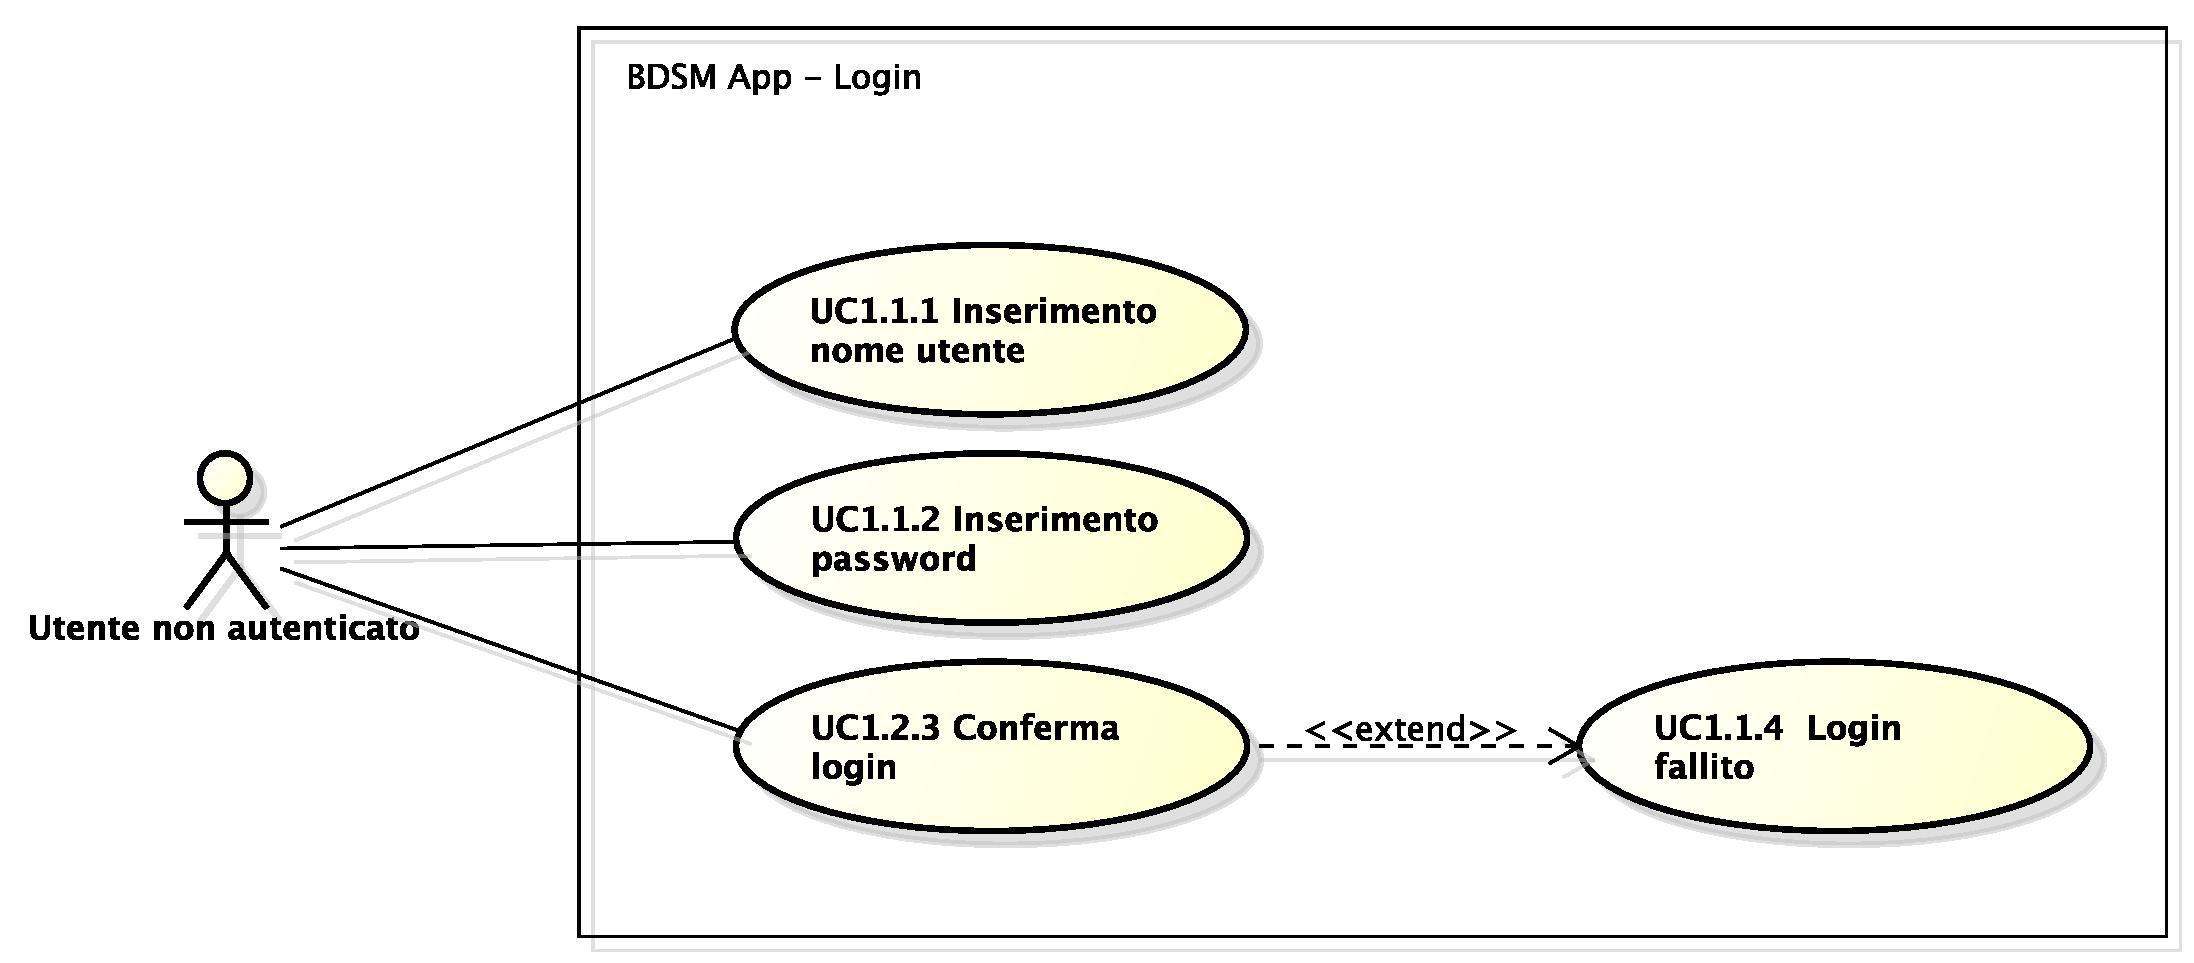
\includegraphics[scale=0.45]{./images/UC1_1.pdf}}
			\caption{D1.2 - Diagramma dell'accesso al sistema}
		\end{figure}
		[TO DO] (descrizione generale)
		% subsubsection accesso_al_sistema (end)

		\subsubsection{D1.3: Visualizzazione documentazione servizi REST} % (fold)
		\label{ssub:visualizzazione_documentazione_servizi_rest}
		\begin{figure}[!htbp]
			\centering
			\centerline{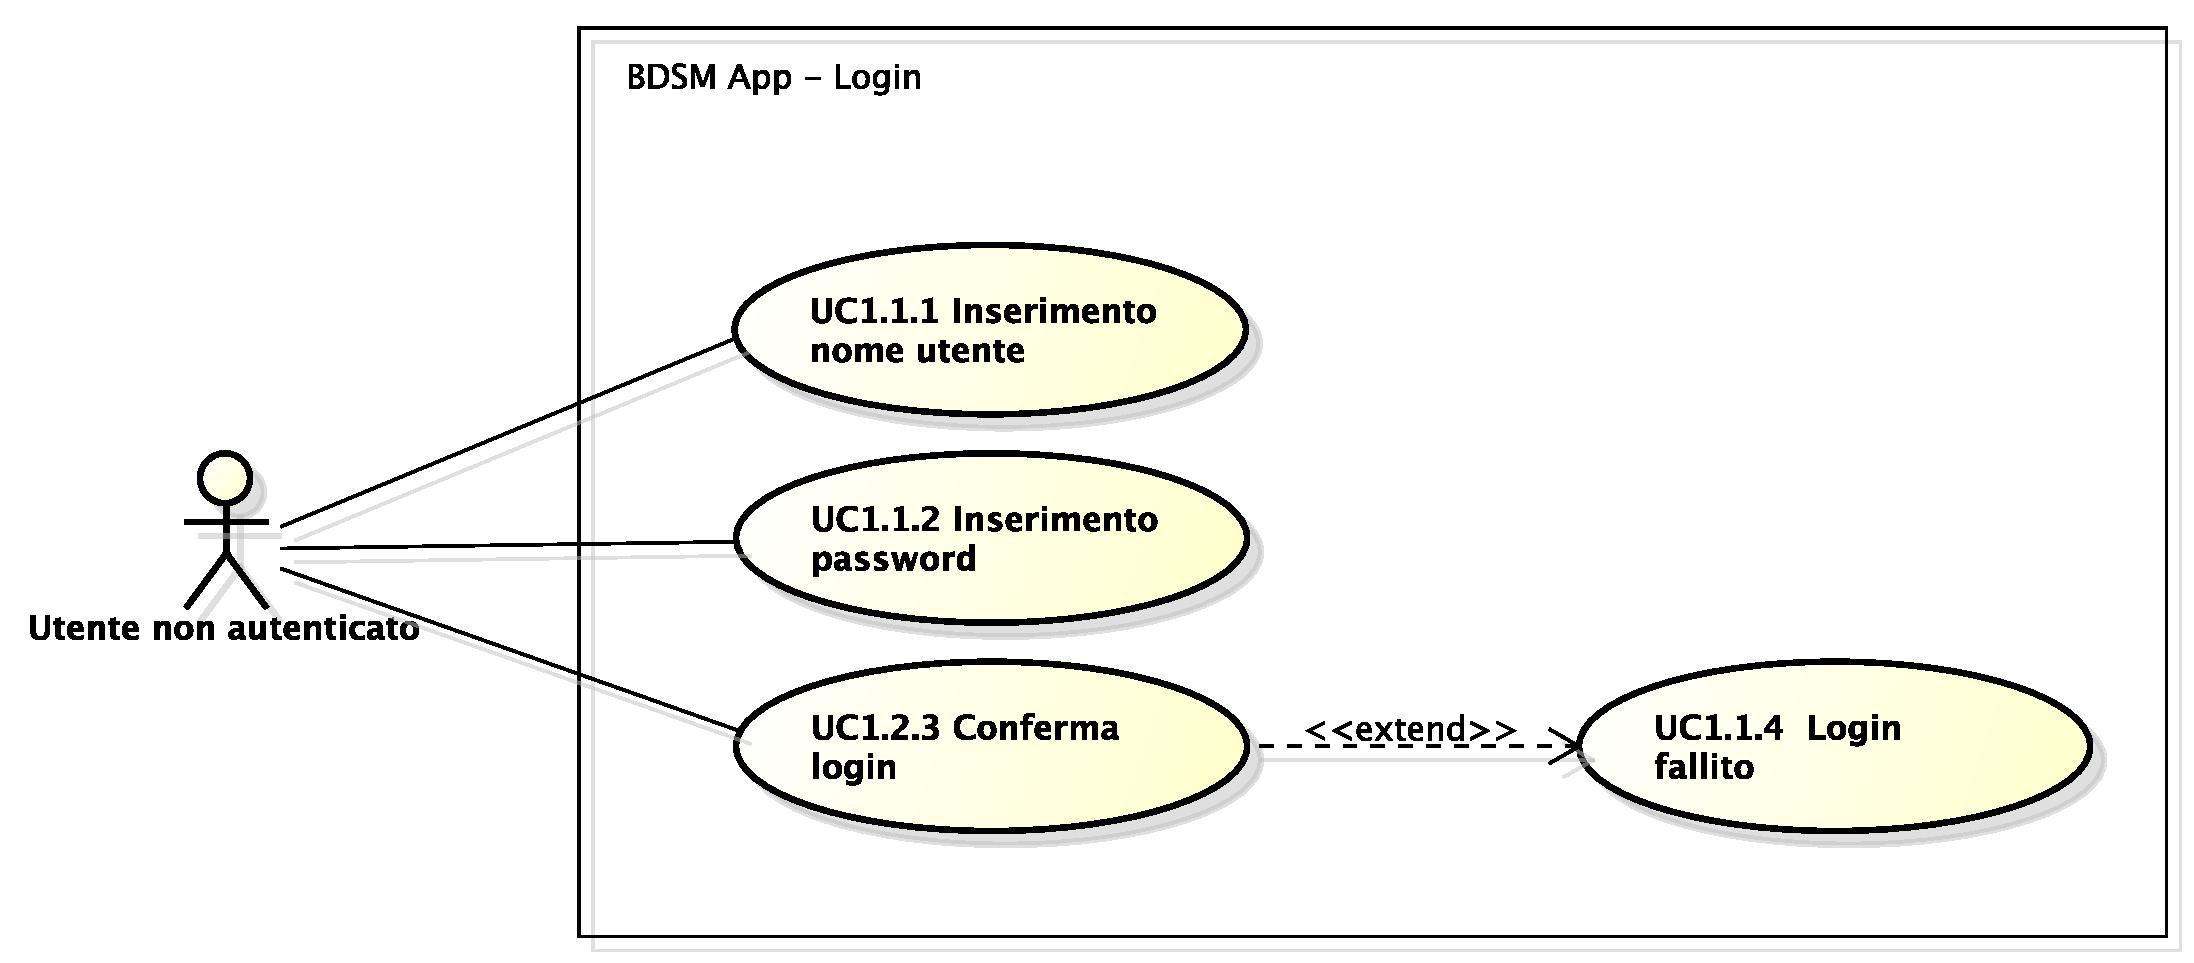
\includegraphics[scale=0.45]{./images/UC1_1.pdf}}
			\caption{D1.3 - Diagramma della visualizzazione documentazione servizi REST}
		\end{figure}
		[TO DO] (descrizione generale)
		% subsubsection visualizzazione_documentazione_servizi_rest (end)

	% subsection utente_non_autenticato (end)

	\pagebreak

	\subsection{Utente autenticato} % (fold)
	\label{sub:utente_autenticato}
	In questa sezione vengono illustrate le attività che un utente autenticato al sistema può compiere.
		\subsubsection{D2: Attività principali dell'utente autenticato} % (fold)
		\label{ssub:attivita_principali_dell_utente_autenticato}
		\begin{figure}[!htbp]
			\centering
			\centerline{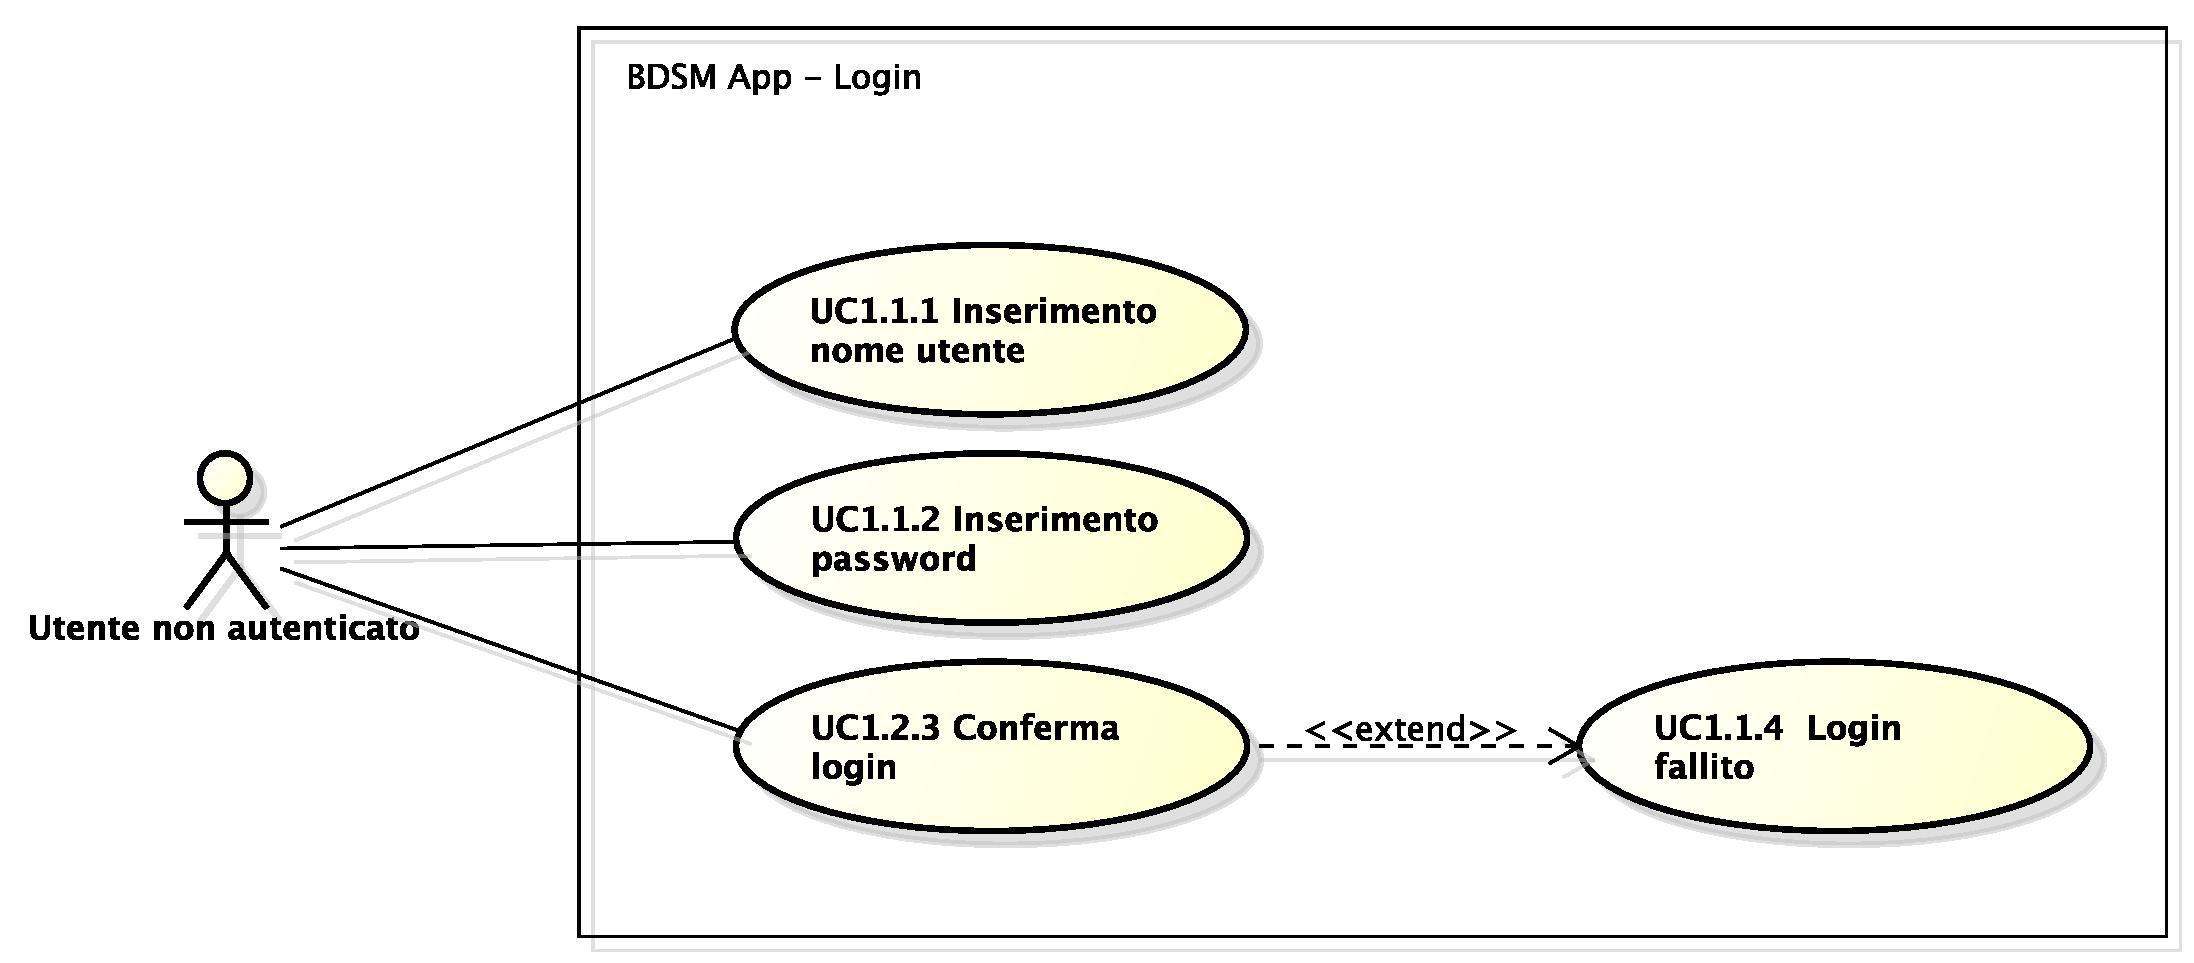
\includegraphics[scale=0.45]{./images/UC1_1.pdf}}
			\caption{D2 - Diagramma delle attività principali dell'utente autenticato}
		\end{figure}
		[TO DO] (descrizione generale e elenco delle attività principali)
		% subsubsection attività_principali_dell_utente_autenticato (end)


		\subsubsection{D2.1: Visualizzazione metriche di una Recipe} % (fold)
		\label{ssub:visualizzazione_metriche_di_una_recipe}
		\label{ssub:registrazione_al_sistema}
		\begin{figure}[!htbp]
			\centering
			\centerline{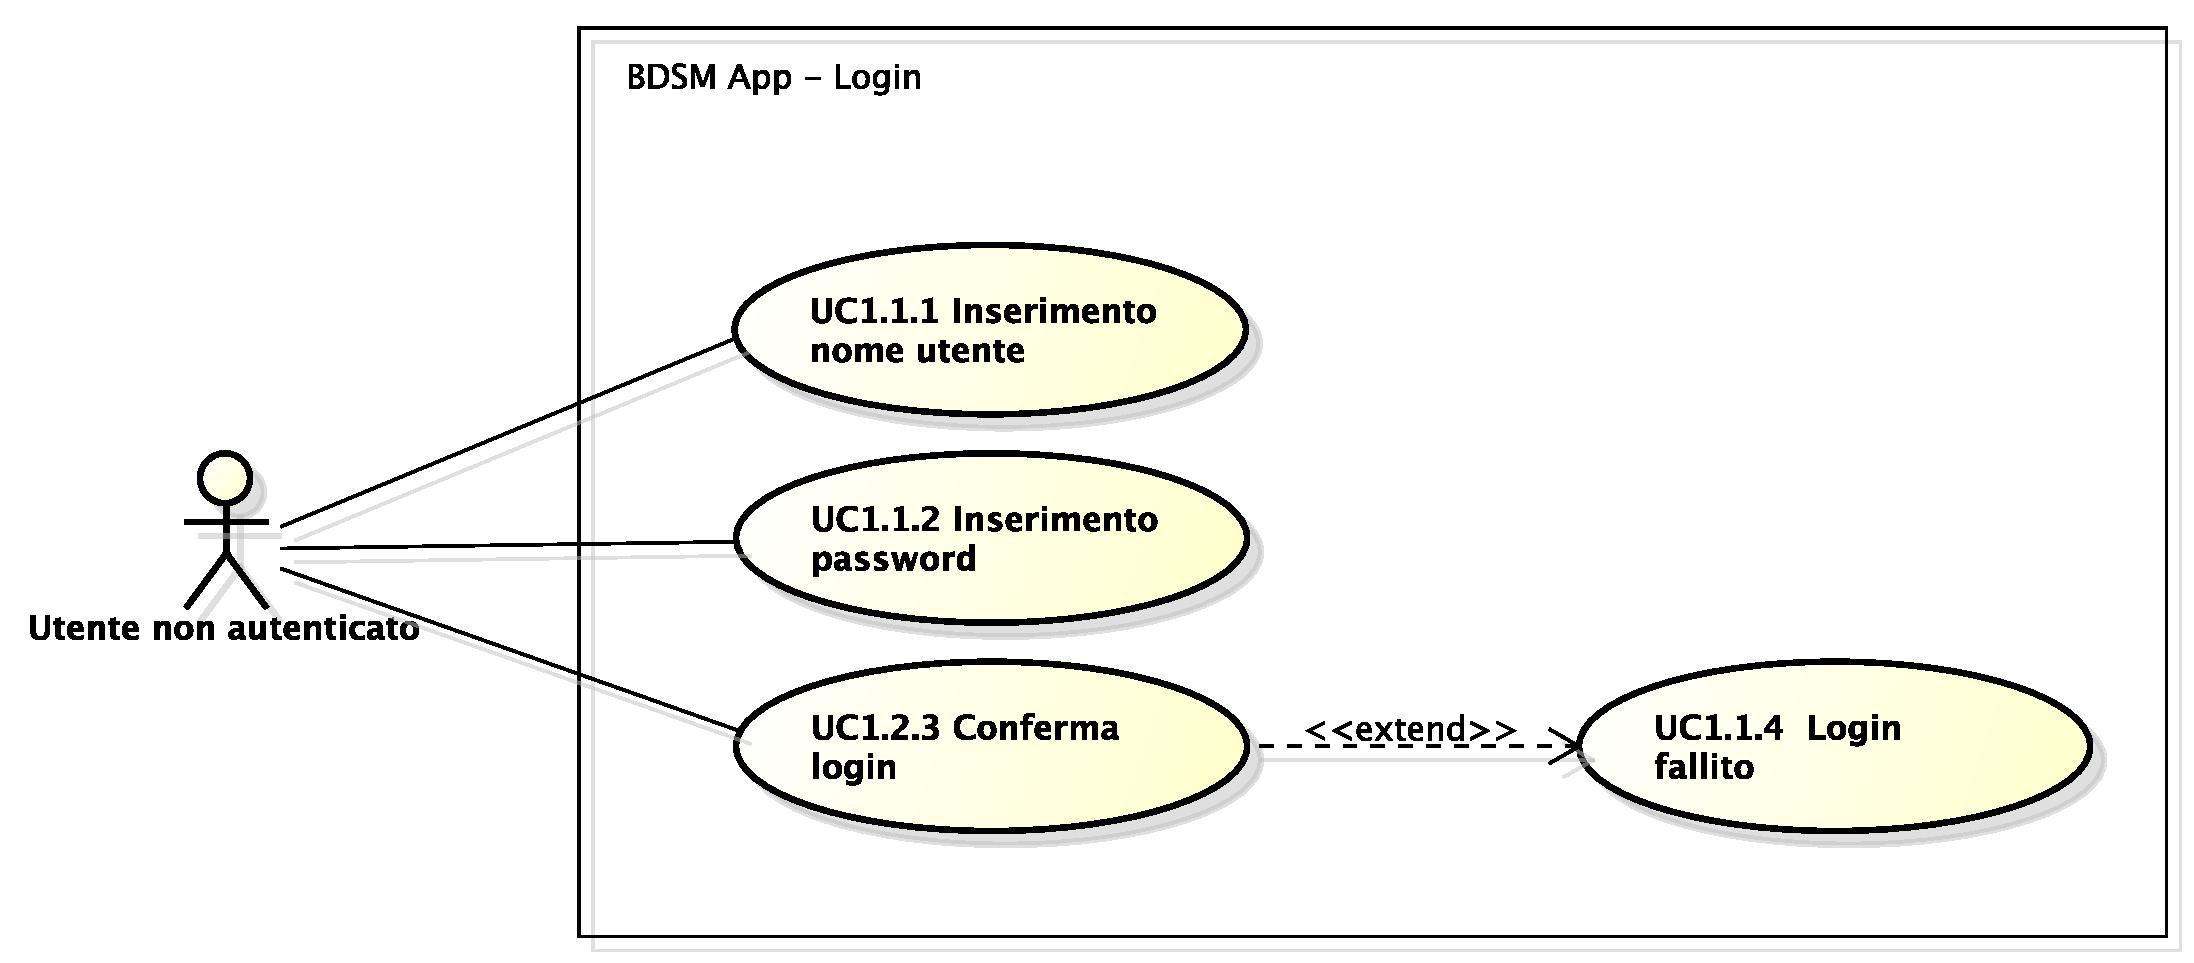
\includegraphics[scale=0.45]{./images/UC1_1.pdf}}
			\caption{D2.1 - Diagramma della visualizzazione metriche di una Recipe}
		\end{figure}
		[TO DO] (descrizione generale)
		% subsubsection visualizzazione_metriche_di_una_recipe (end)

		\subsubsection{D2.1.1: Visualizzazione delle View di una metrica} % (fold)
		\label{ssub:visualizzazione_view_di_una_metrica}
		\begin{figure}[!htbp]
			\centering
			\centerline{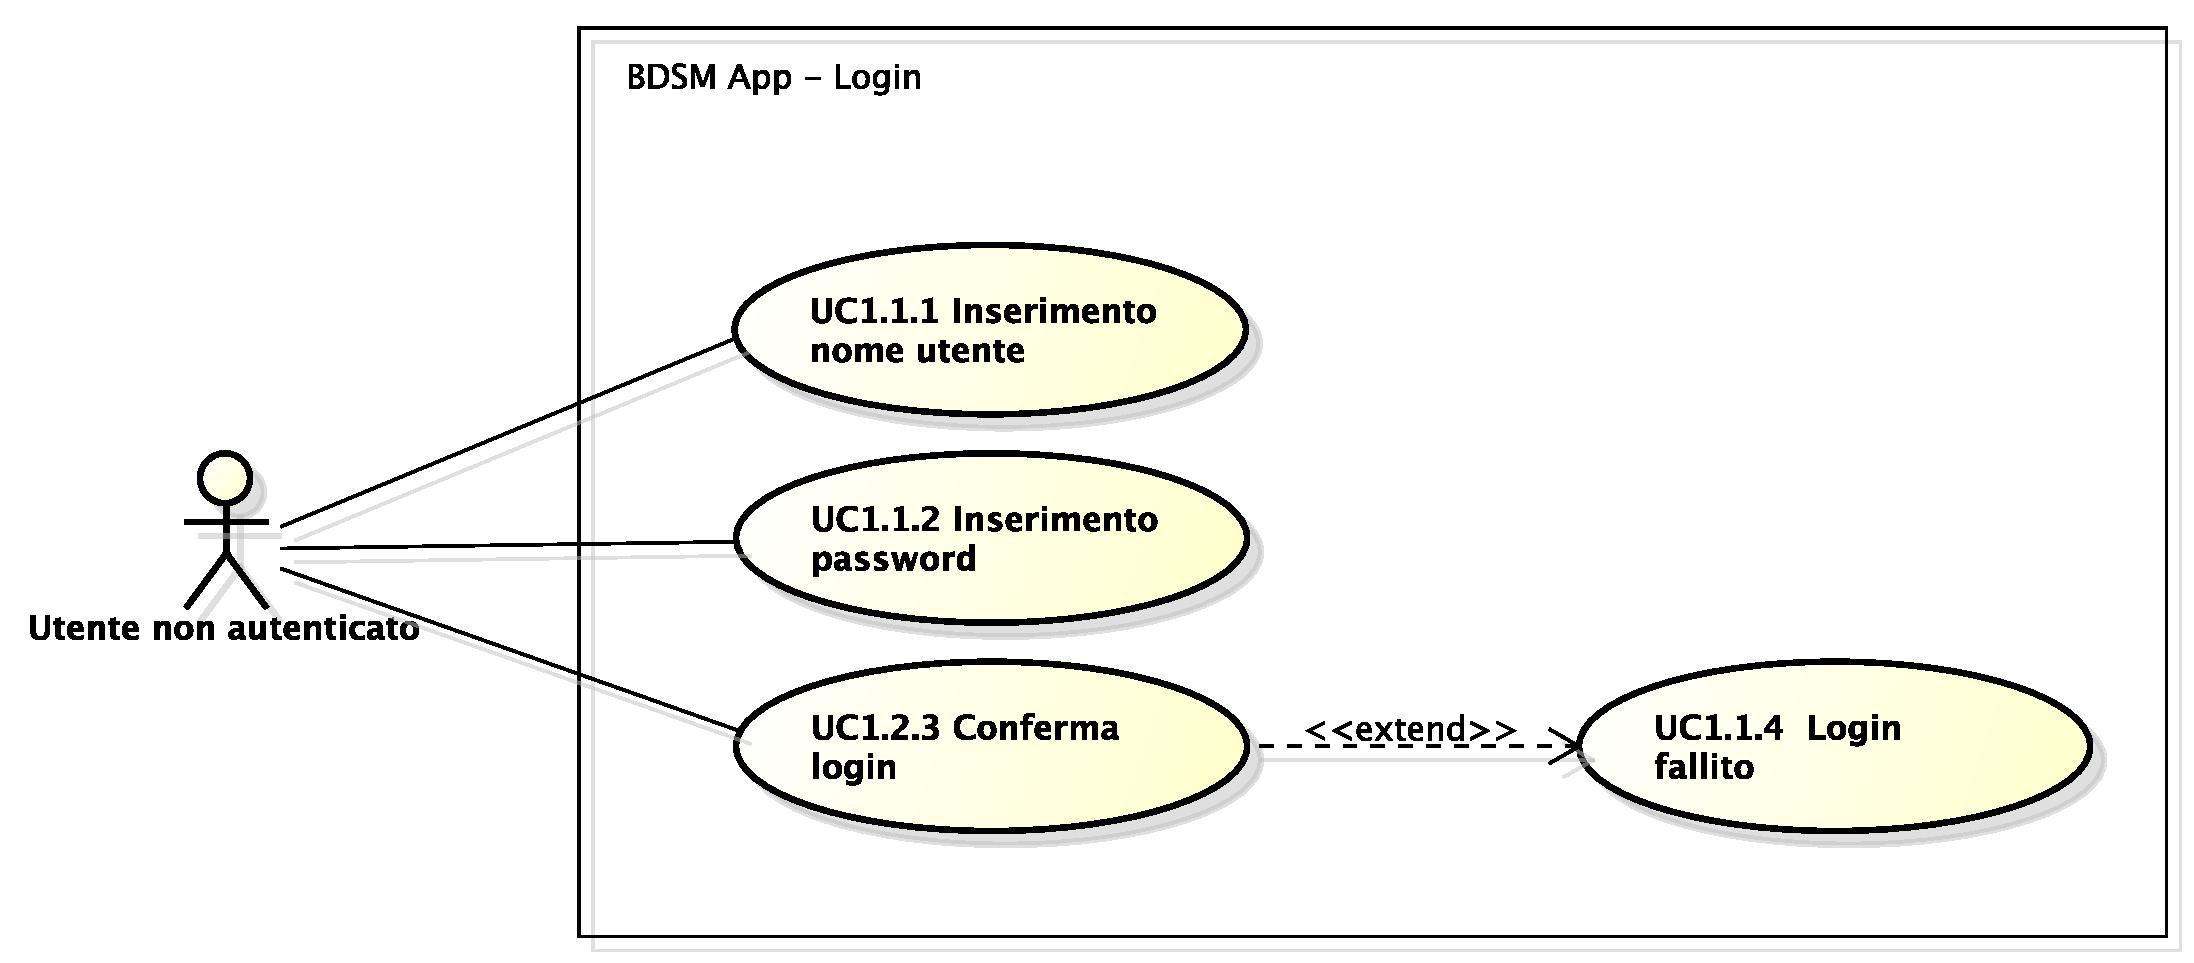
\includegraphics[scale=0.45]{./images/UC1_1.pdf}}
			\caption{D2.1.1 - Diagramma della visualizzazione delle View di una metrica}
		\end{figure}
		[TO DO] (descrizione generale)
		% subsubsection visualizzazione_view_di_una_metrica (end)

		\subsubsection{D2.2: Confronto tra metriche di una Recipe} % (fold)
		\label{ssub:confronto_tra_metriche_di_una_recipe}
		\begin{figure}[!htbp]
			\centering
			\centerline{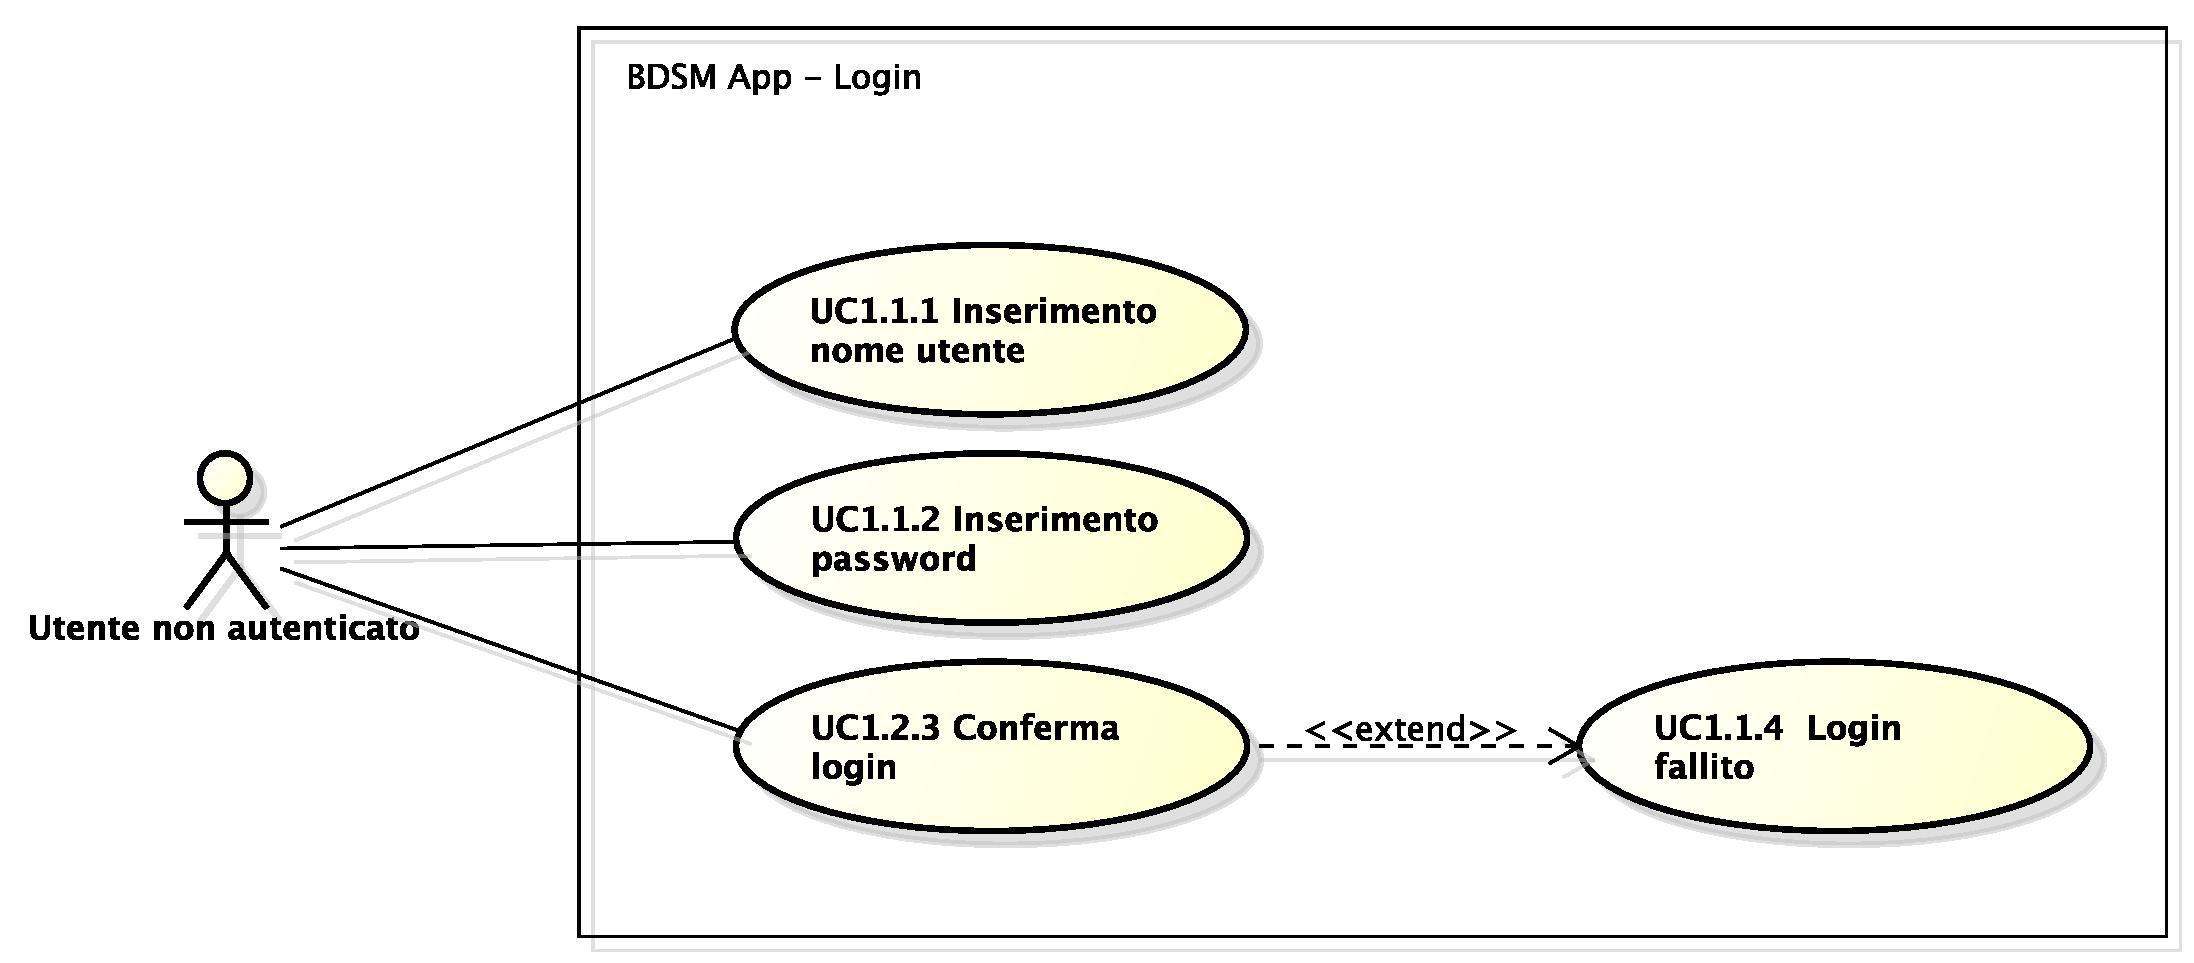
\includegraphics[scale=0.45]{./images/UC1_1.pdf}}
			\caption{D2.2 - Diagramma del confronto tra metriche di una Recipe}
		\end{figure}
		[TO DO] (descrizione generale)
		% subsubsection confronto_tra_metriche_di_una_recipe (end)

		\subsubsection{D2.3: Visualizzazione dei preferiti} % (fold)
		\label{ssub:visualizzazione_dei_preferiti}
		\begin{figure}[!htbp]
			\centering
			\centerline{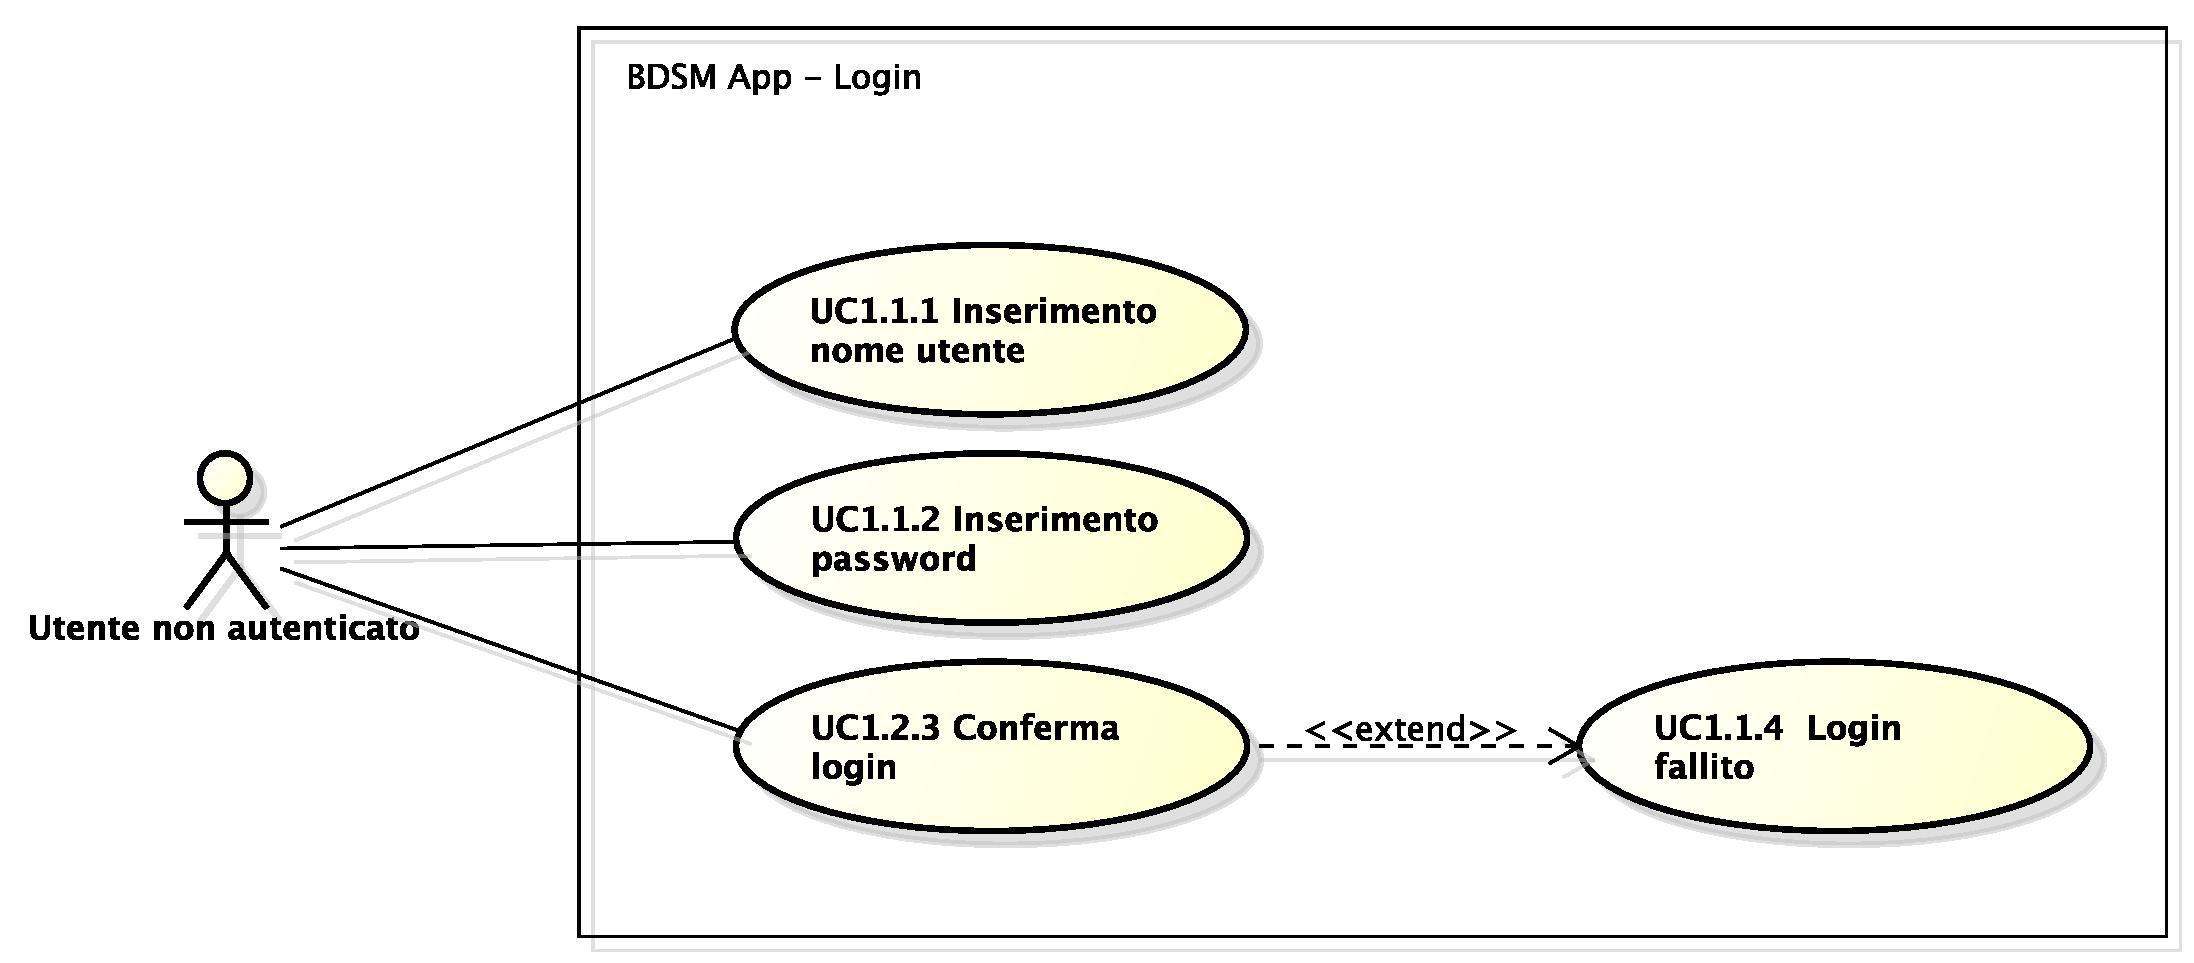
\includegraphics[scale=0.45]{./images/UC1_1.pdf}}
			\caption{D2.3 - Diagramma della visualizzazione dei preferiti}
		\end{figure}
		[TO DO] (descrizione generale)
		% subsubsection visualizzazione_dei_preferiti (end)

		\subsubsection{D2.4: Richiesta di una nuova Recipe} % (fold)
		\label{ssub:richiesta_di_una_nuova_recipe}
		\begin{figure}[!htbp]
			\centering
			\centerline{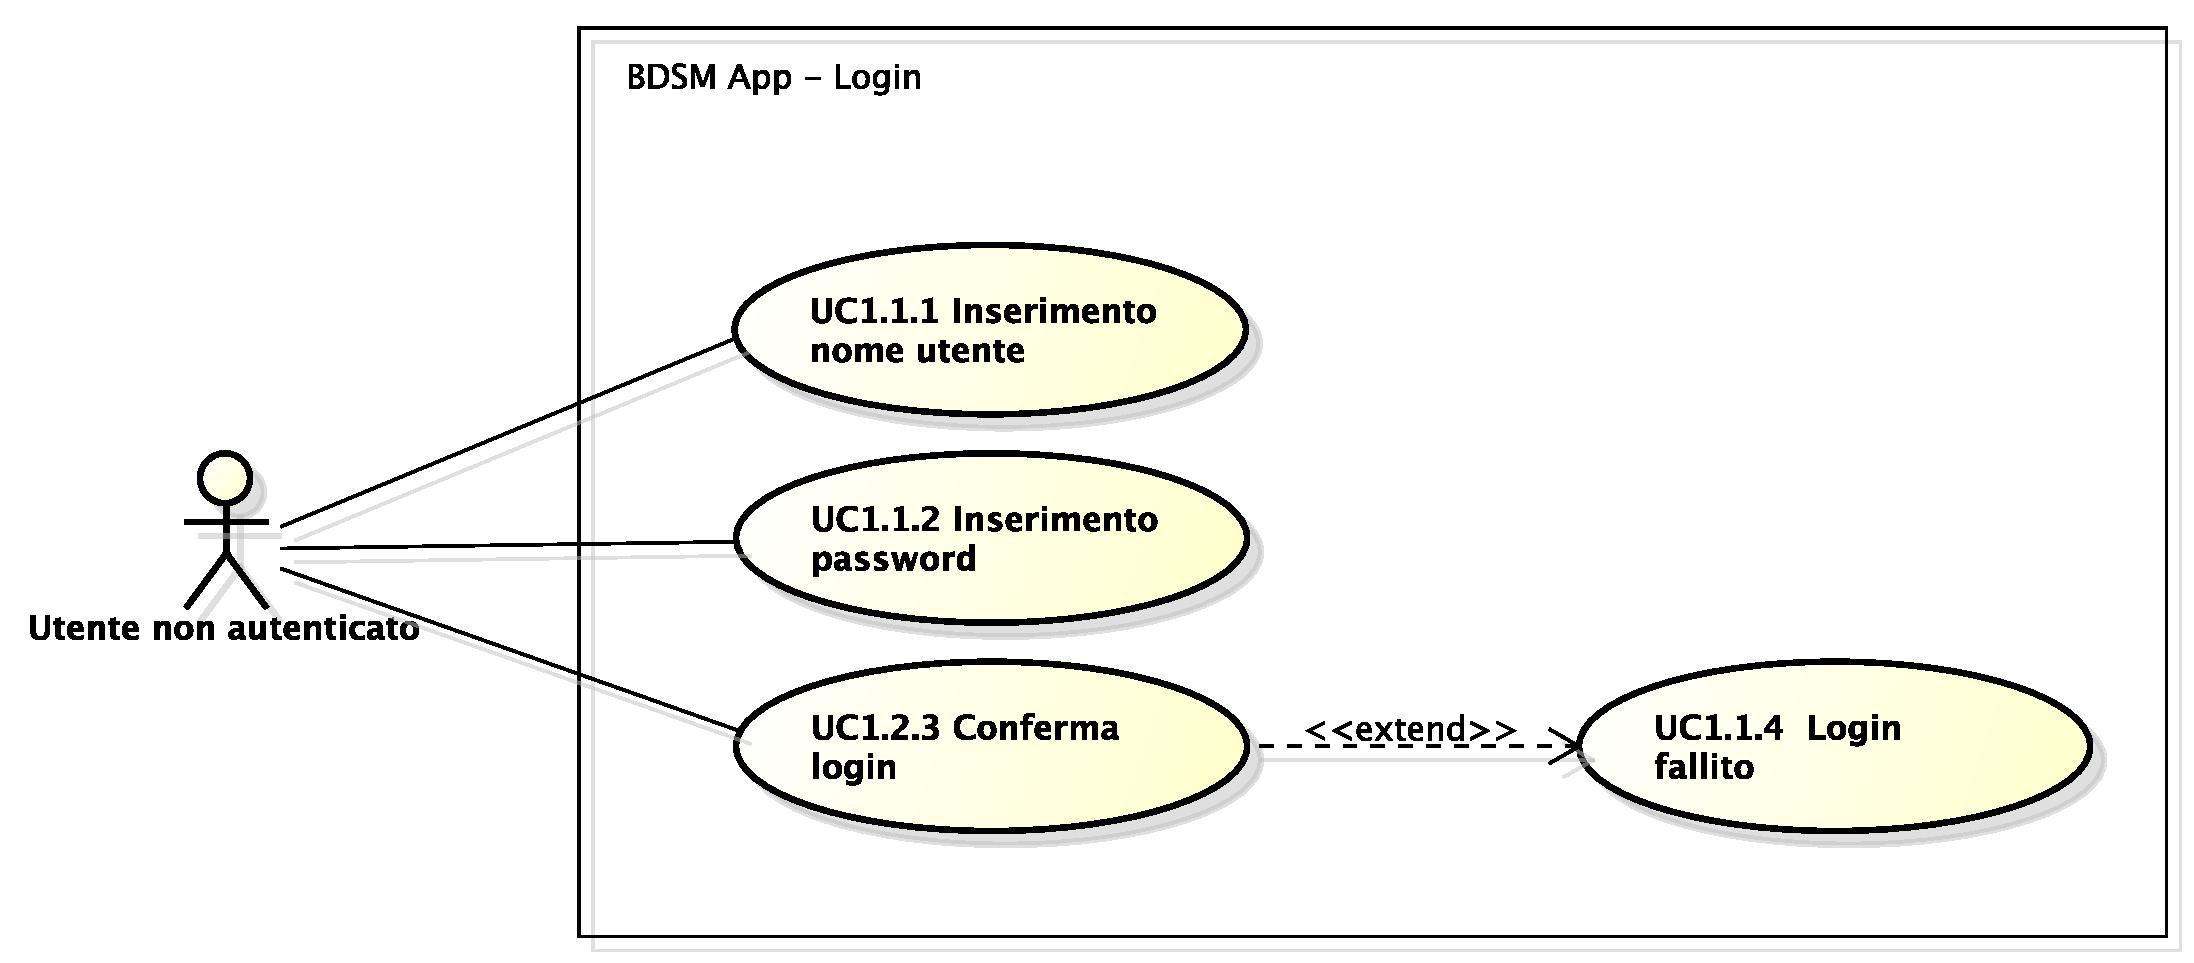
\includegraphics[scale=0.45]{./images/UC1_1.pdf}}
			\caption{D2.4 - Diagramma della richiesta di una nuova Recipe}
		\end{figure}
		[TO DO] (descrizione generale)
		% subsubsection richiesta_di_una_nuova_recipe (end)

		\subsubsection{D2.5: Gestione token di accesso} % (fold)
		\label{ssub:gestione_token_di_accesso}
		\begin{figure}[!htbp]
			\centering
			\centerline{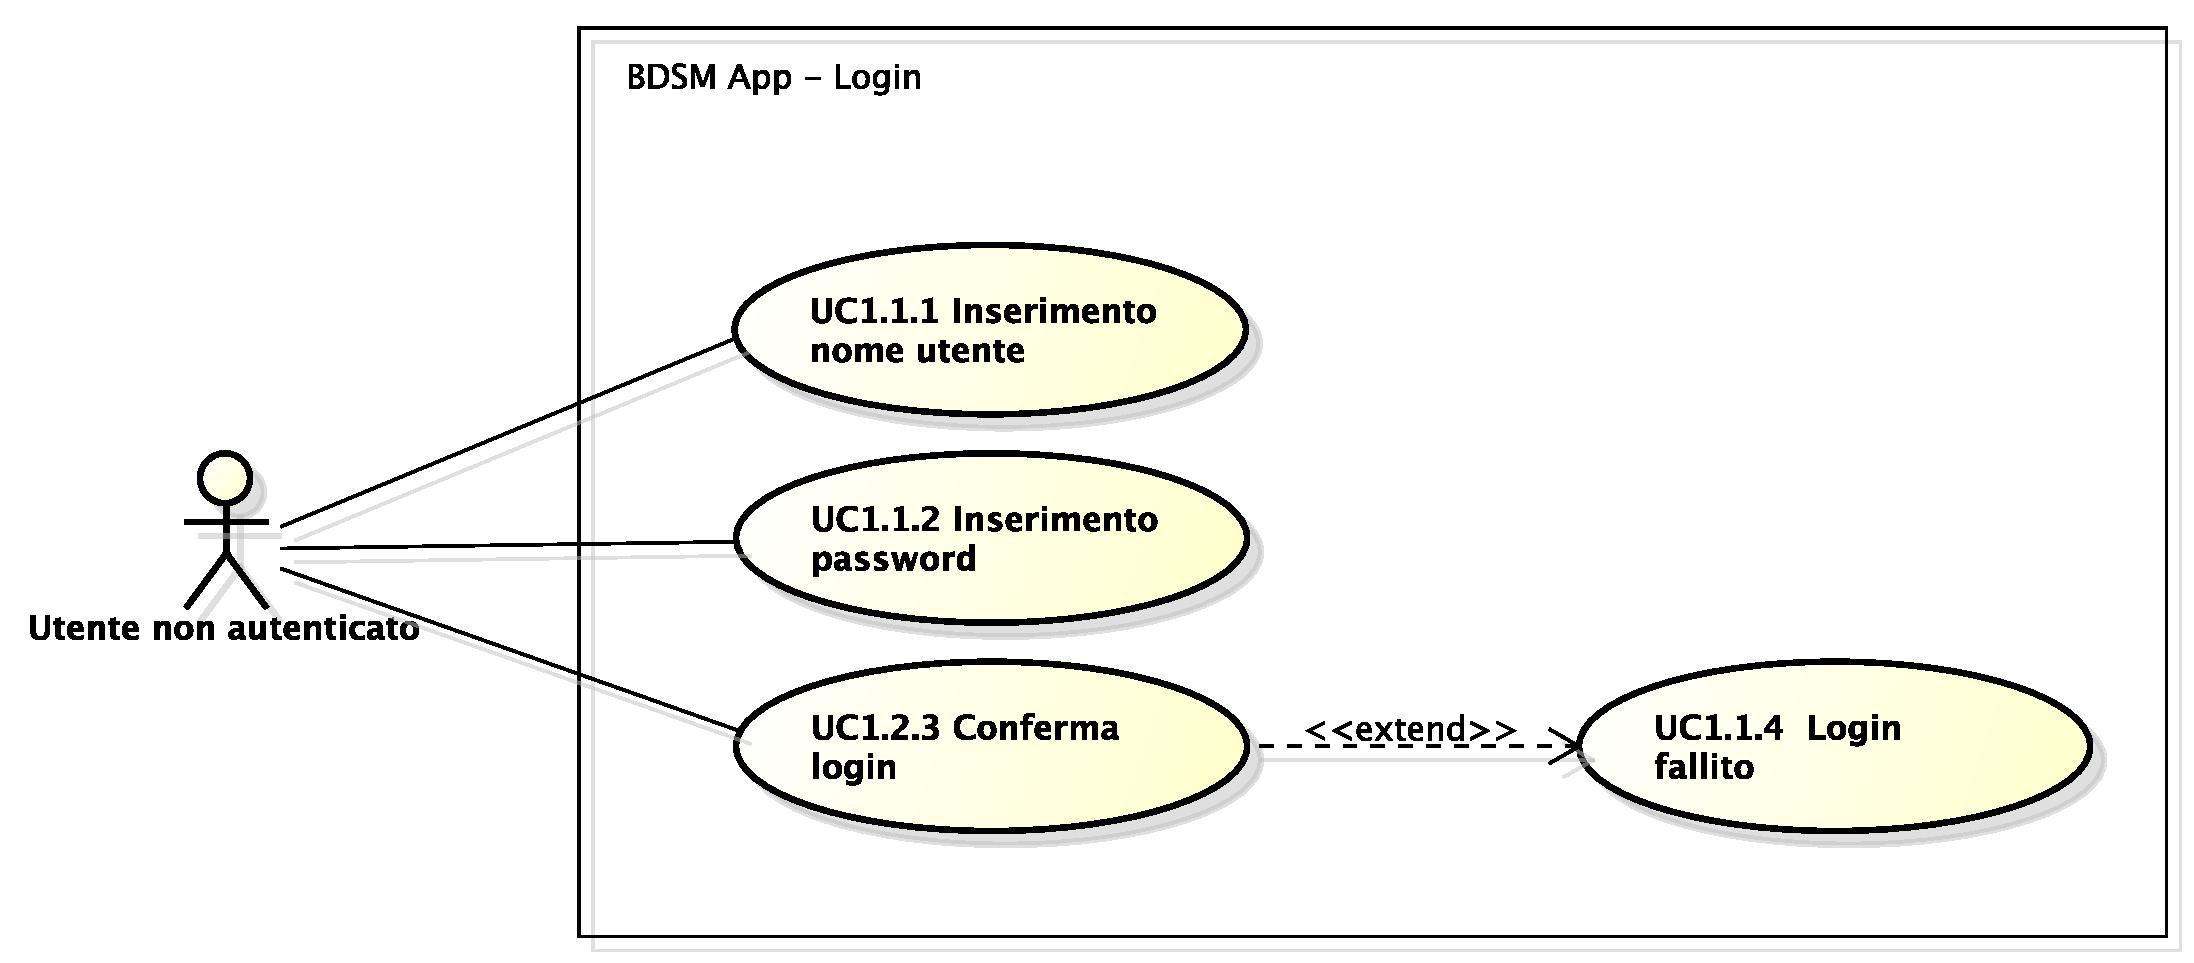
\includegraphics[scale=0.45]{./images/UC1_1.pdf}}
			\caption{D2.5 - Diagramma della gestione del token di accesso}
		\end{figure}
		[TO DO] (descrizione generale)
		% subsubsection gestione_token_di_accesso (end)

		\subsubsection{D2.6: Visualizzazione dettagli utente} % (fold)
		\label{ssub:visualizzazione_dettagli_utente}
		\begin{figure}[!htbp]
			\centering
			\centerline{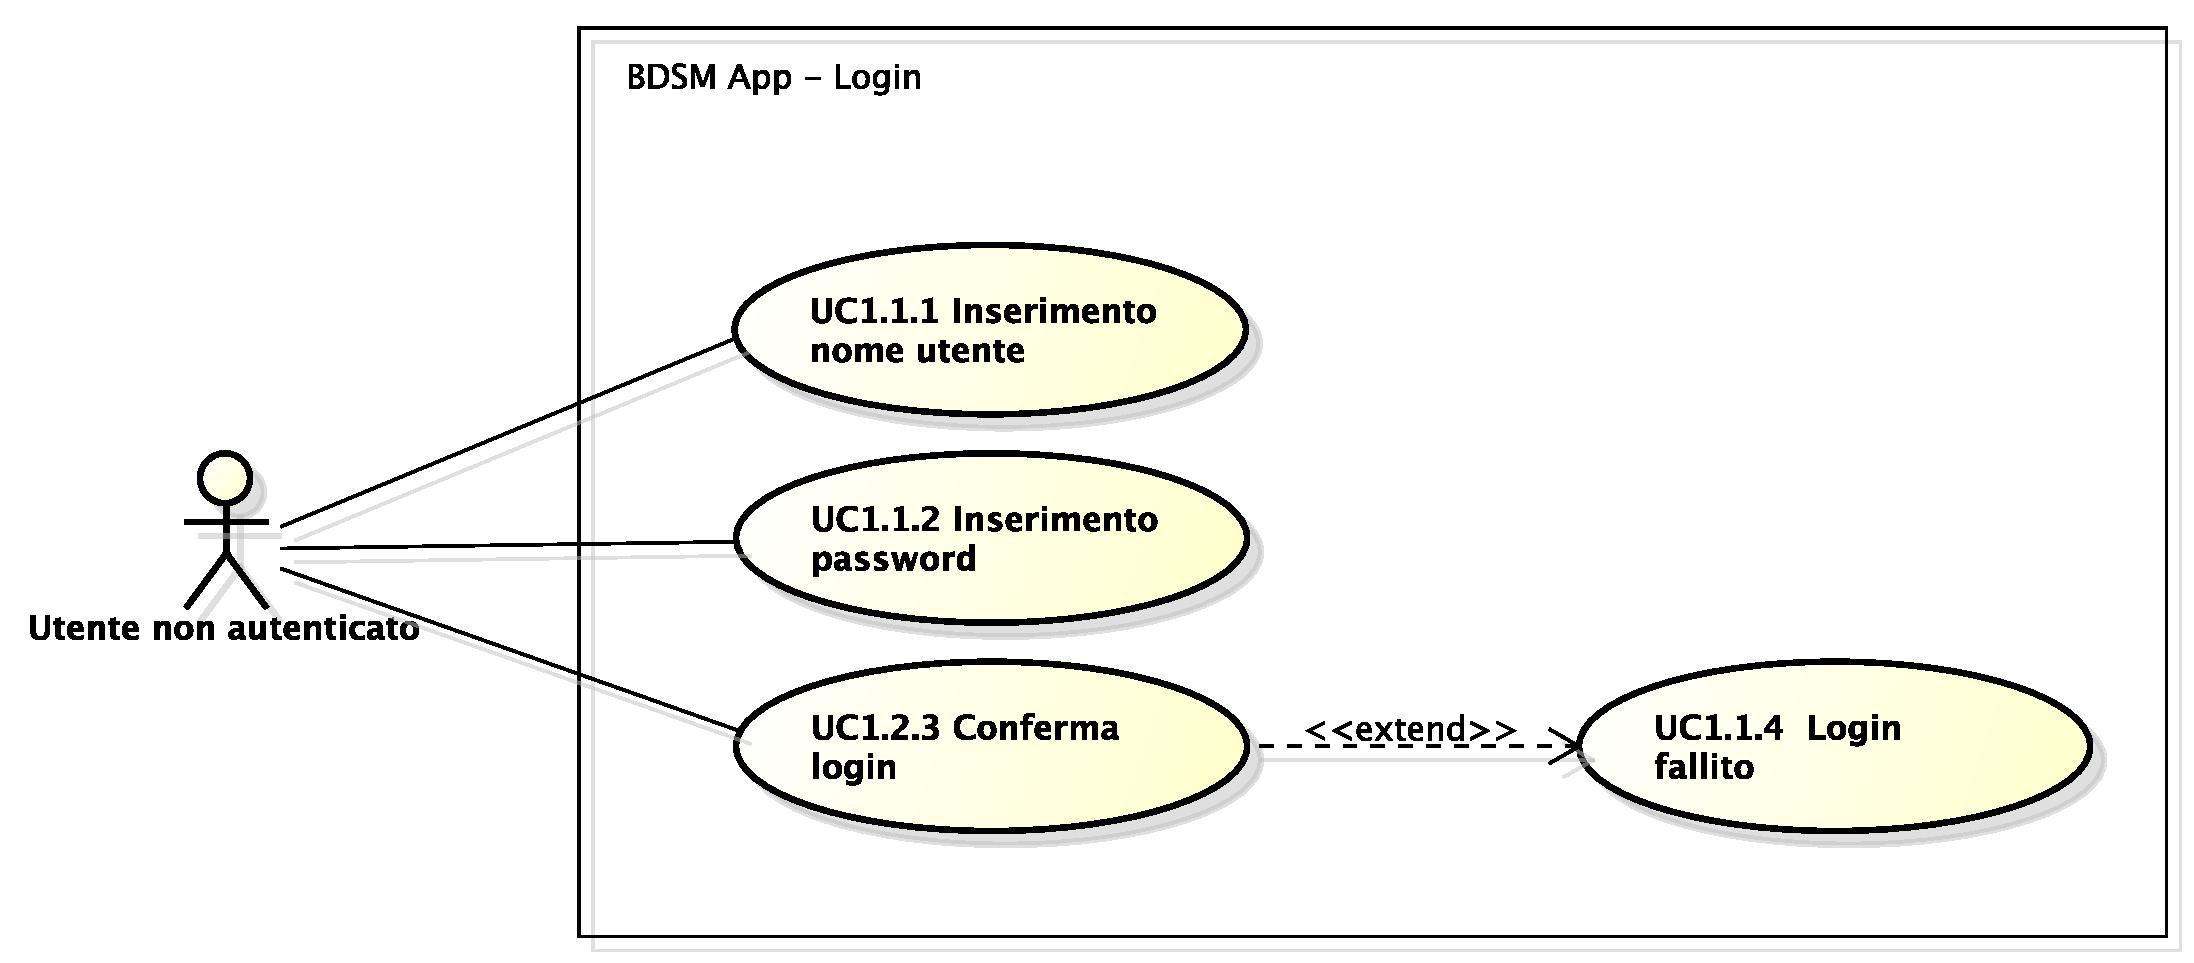
\includegraphics[scale=0.45]{./images/UC1_1.pdf}}
			\caption{D2.6 - Diagramma della visualizzazione dettagli utente}
		\end{figure}
		[TO DO] (descrizione generale)
		% subsubsection visualizzazione_dettagli_utente (end)

		\subsubsection{D2.7: Modifica dei dati utente} % (fold)
		\label{ssub:modifica_dei_dati_utente}
		\begin{figure}[!htbp]
			\centering
			\centerline{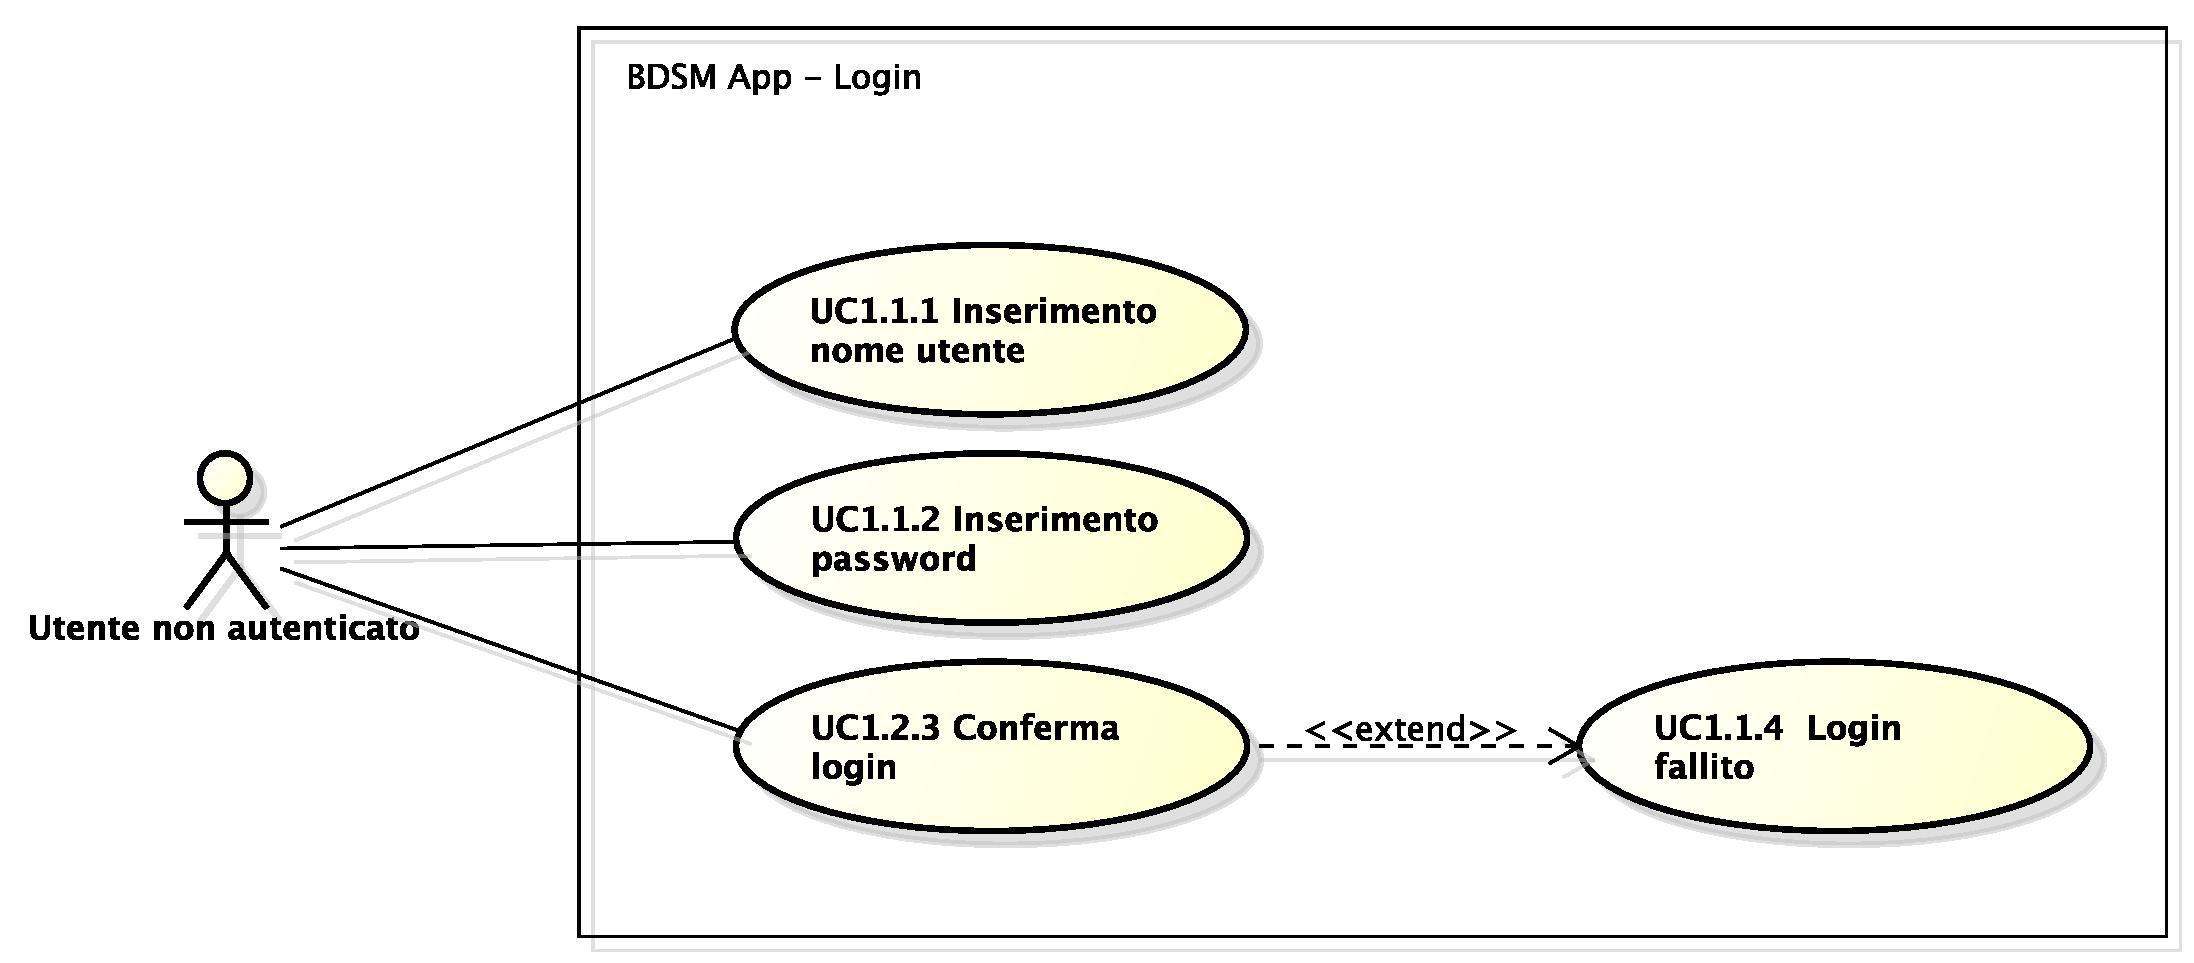
\includegraphics[scale=0.45]{./images/UC1_1.pdf}}
			\caption{D2.7 - Diagramma della modifica dei dati utente}
		\end{figure}
		[TO DO] (descrizione generale)
		% subsubsection modifica_dei_dati_utente (end)

		\subsubsection{D.7.1: Modifica della password} % (fold)
		\label{ssub:modifica_della_password}
		\begin{figure}[!htbp]
			\centering
			\centerline{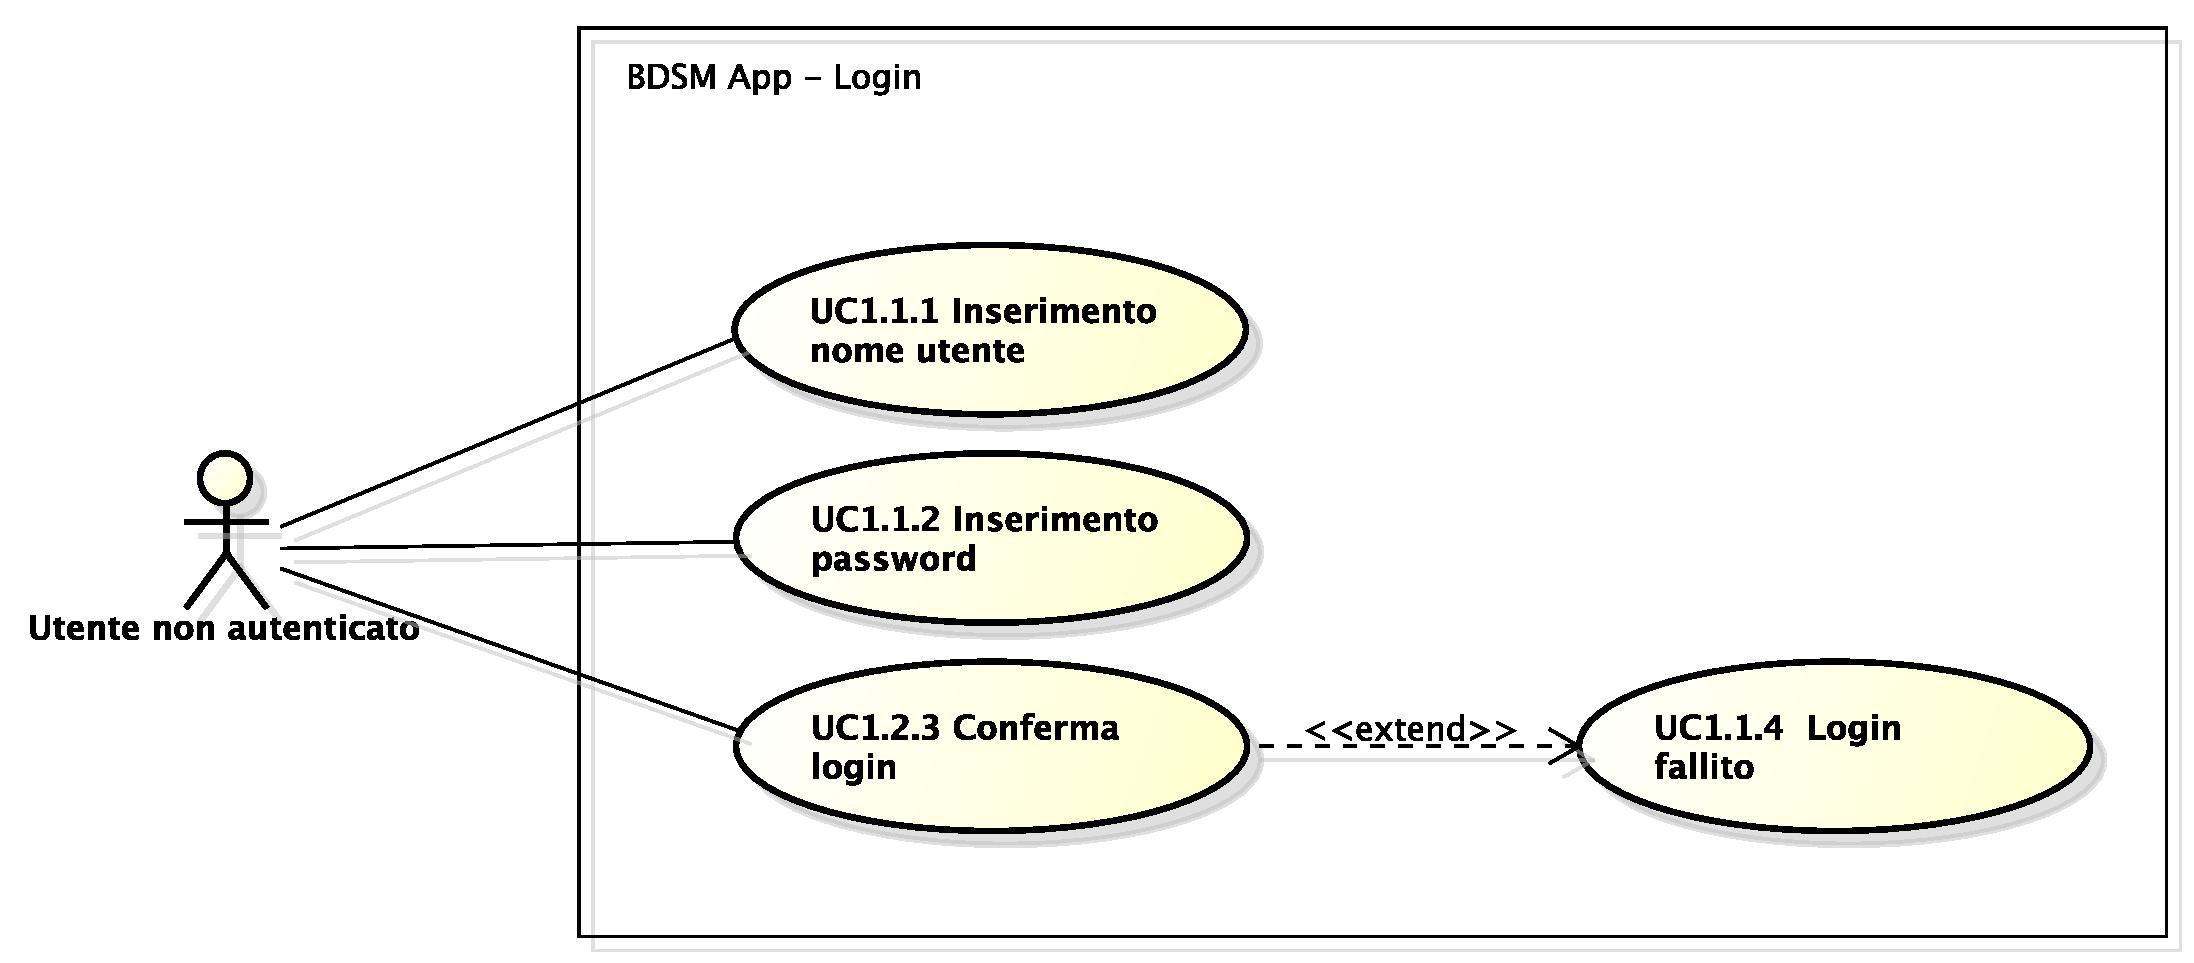
\includegraphics[scale=0.45]{./images/UC1_1.pdf}}
			\caption{D2.7.1 - Diagramma della modifica della password}
		\end{figure}
		[TO DO] (descrizione generale)
		% subsubsection modifica_della_password (end)

	% subsection utente_autenticato (end)

	\pagebreak



	\subsection{Utente amministratore} % (fold)
	\label{sub:utente_amministratore}
	In questa sezione vengono illustrate le attività che un amministratore del sistema può compiere. L'utente amministratore oltre alle suddette potrà svolgere anche tutte le attività presenti nella sezione \ref{ssub:attivita_principali_dell_utente_autenticato}.
		\subsubsection{D3: Attività principali dell'utente amministratore} % (fold)
		\label{ssub:attivita_principali_dell_utente_amministratore}
		\begin{figure}[!htbp]
			\centering
			\centerline{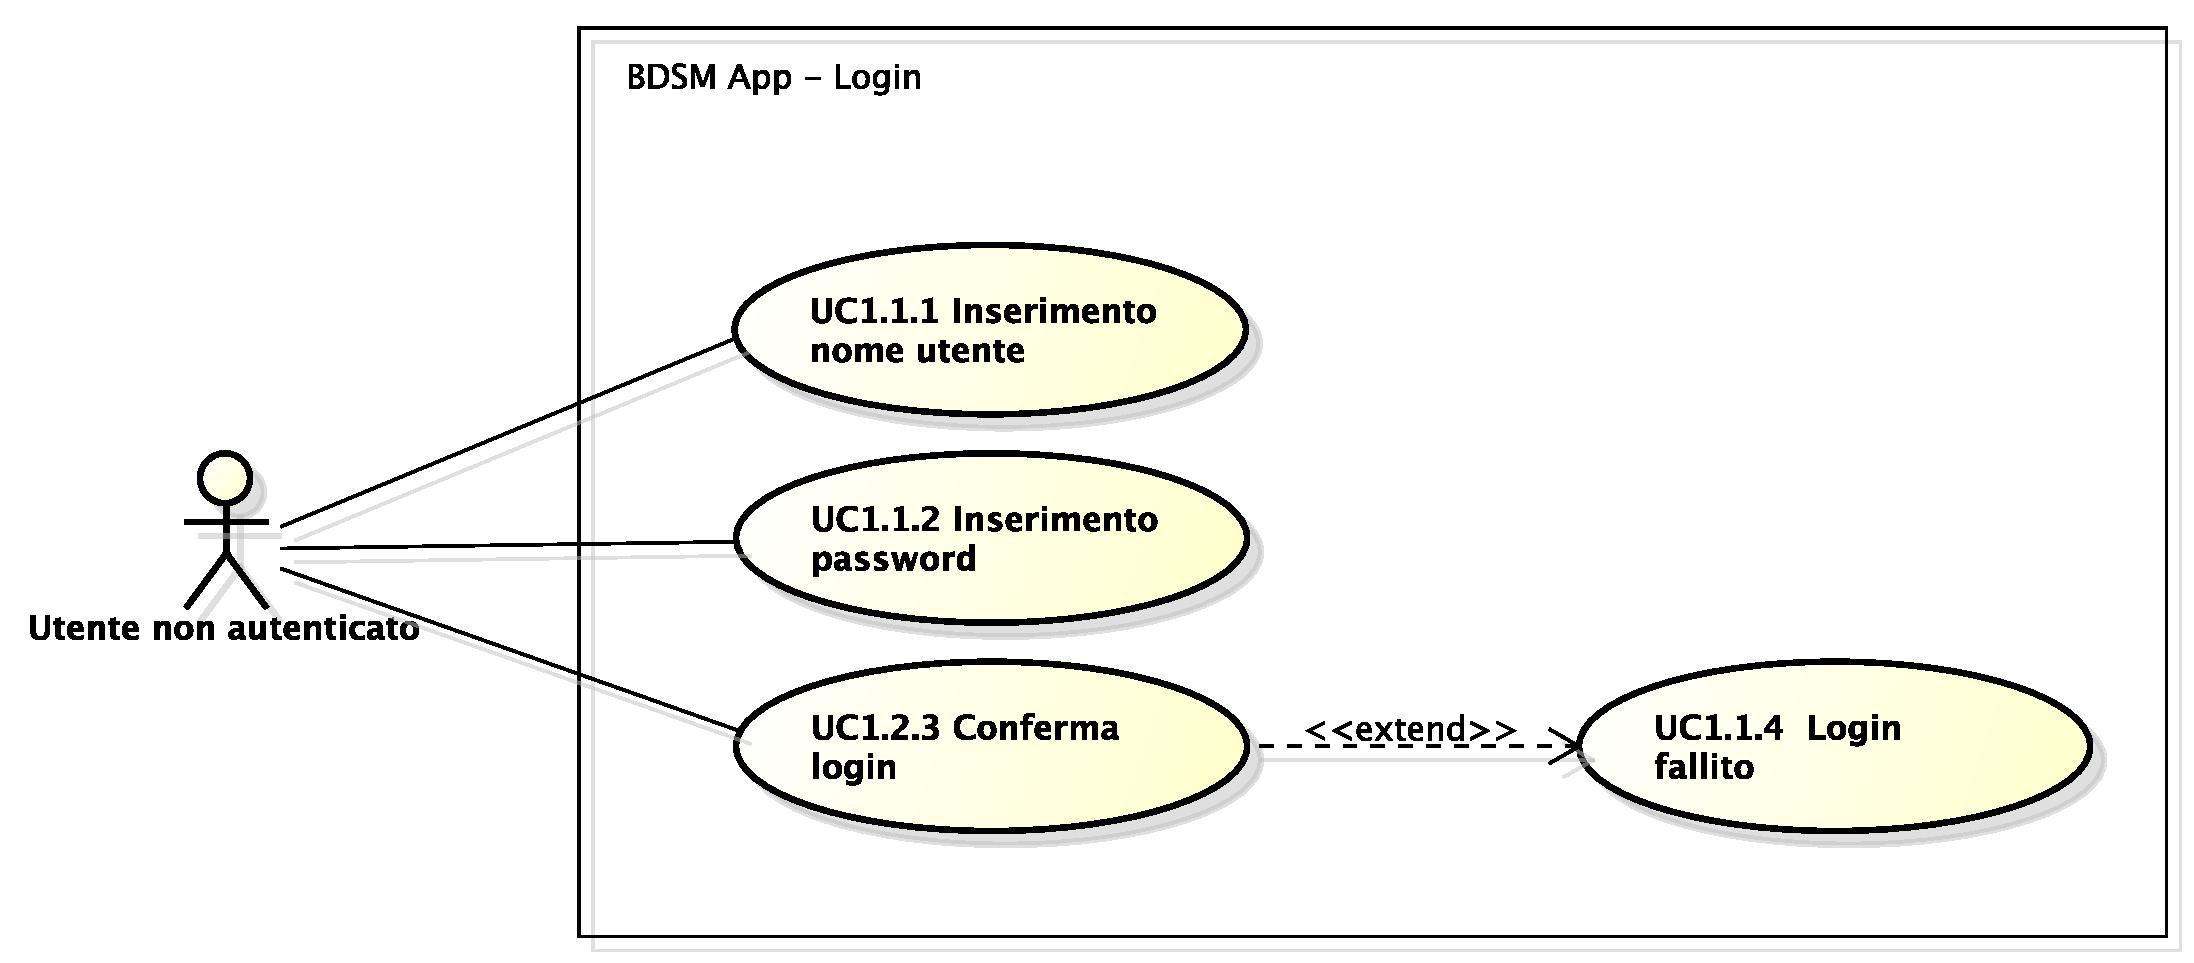
\includegraphics[scale=0.45]{./images/UC1_1.pdf}}
			\caption{D3 - Diagramma delle attività principali dell'utente amministratore}
		\end{figure}
		[TO DO] (descrizione generale e elenco delle attività principali)

		% subsubsection attività_principali_dell_utente_amministratore (end)


		\subsubsection{D3.1: Inserimento nuova Recipe} % (fold)
		\label{ssub:inserimento_nuova_recipe}
		\begin{figure}[!htbp]
			\centering
			\centerline{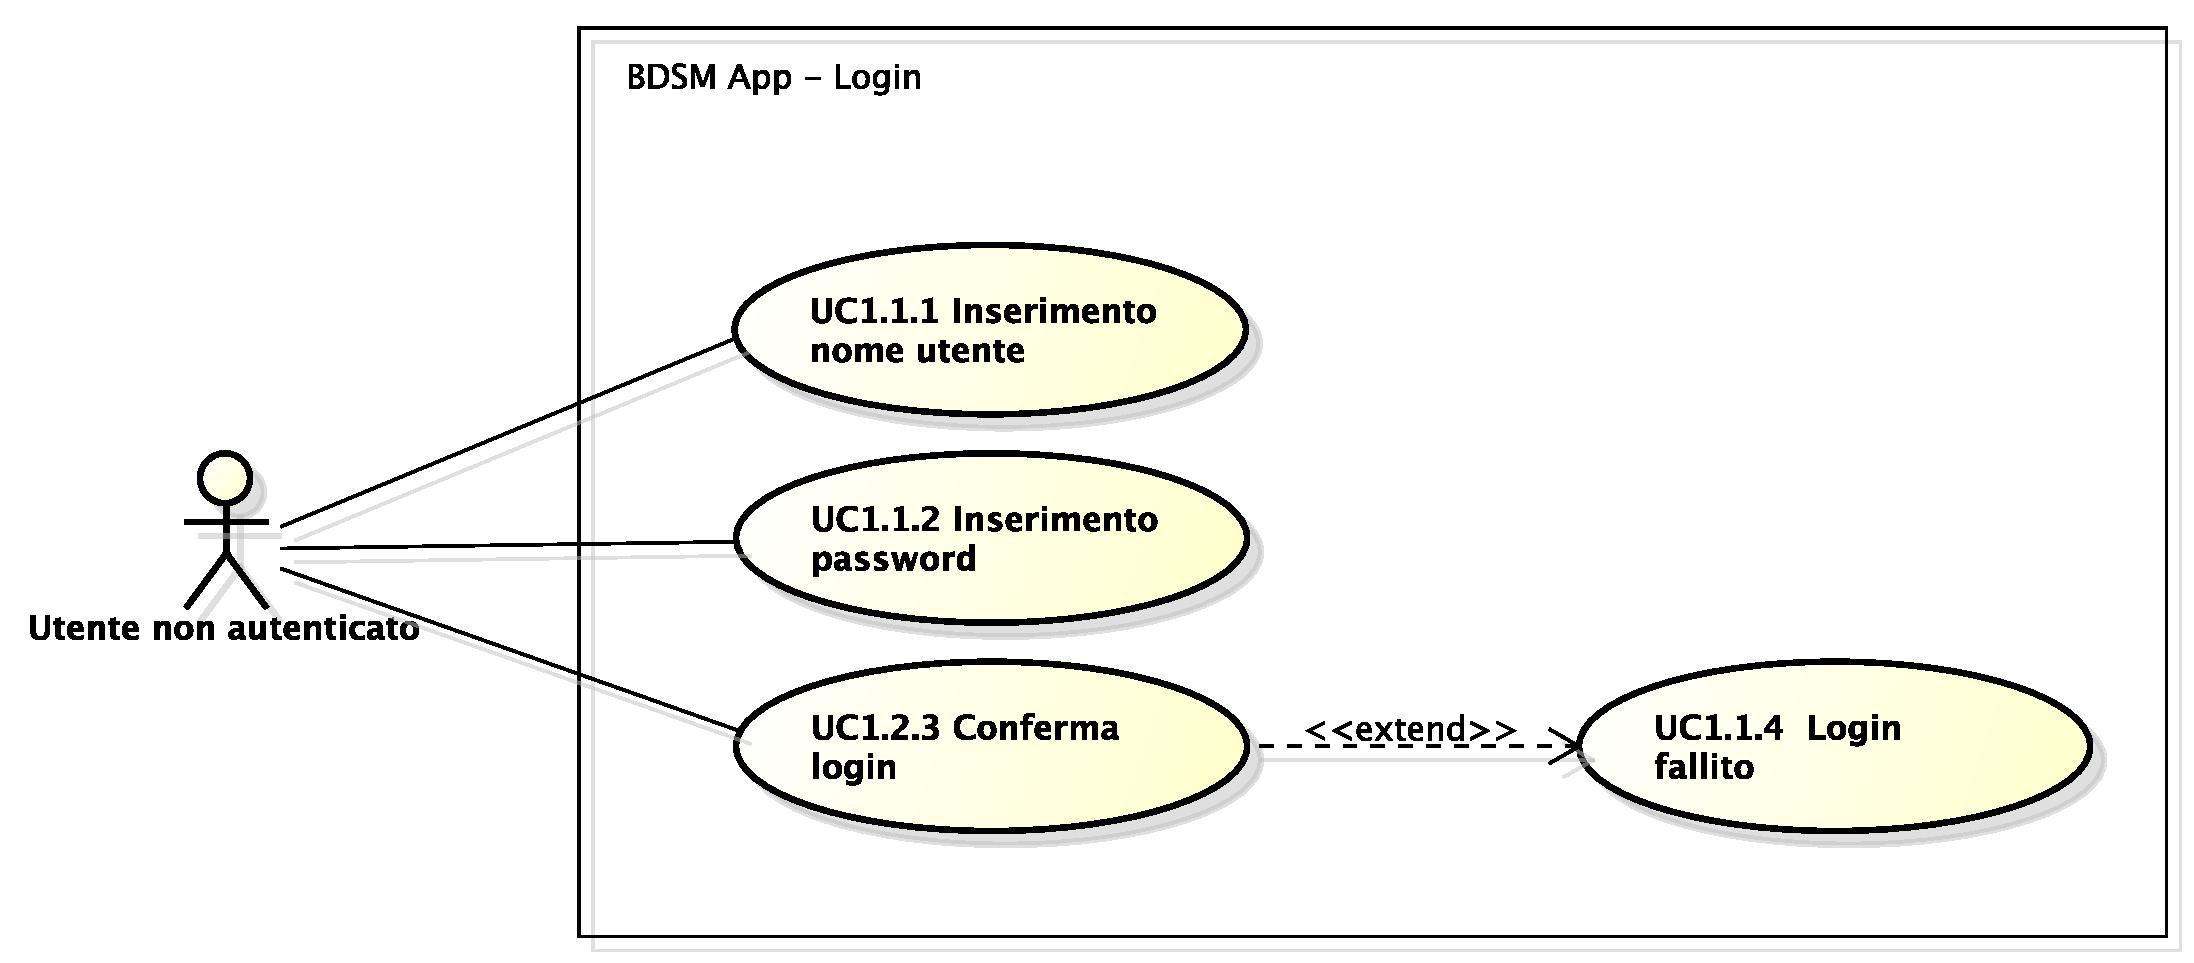
\includegraphics[scale=0.45]{./images/UC1_1.pdf}}
			\caption{D3.1 - Diagramma dell'inserimento di una nuova Recipe}
		\end{figure}
		[TO DO] (descrizione generale)
		% subsubsection inserimento_nuova_recipe (end)


		\subsubsection{D3.2: Gestione richieste Recipe} % (fold)
		\label{ssub:gestione_richieste_recipe}
		\begin{figure}[!htbp]
			\centering
			\centerline{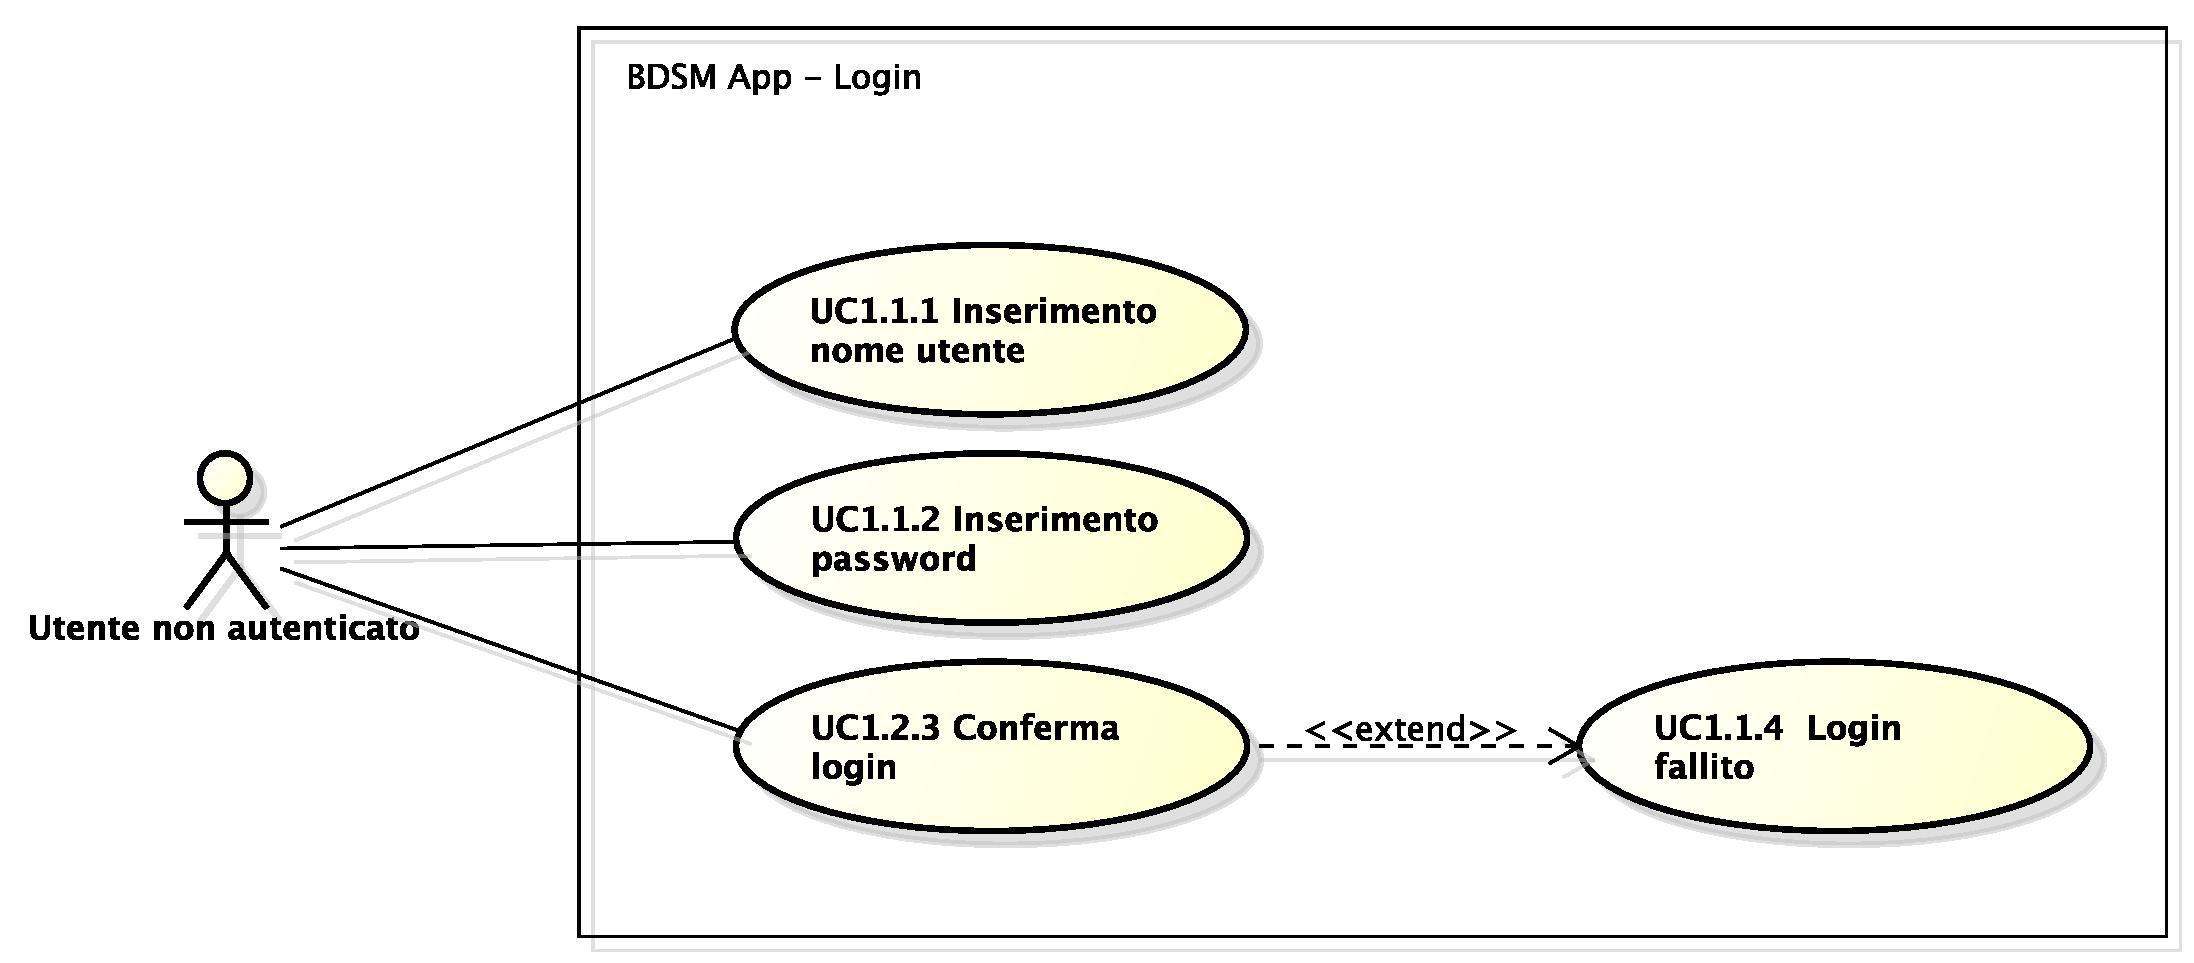
\includegraphics[scale=0.45]{./images/UC1_1.pdf}}
			\caption{D3.2 - Diagramma della gestione delle richieste Recipe}
		\end{figure}
		[TO DO] (descrizione generale)
		% subsubsection gestione_richieste_recipe (end)

		\subsubsection{D3.3: Amministrazione degli utenti} % (fold)
		\label{ssub:amministrazione_degli_utenti}
		\begin{figure}[!htbp]
			\centering
			\centerline{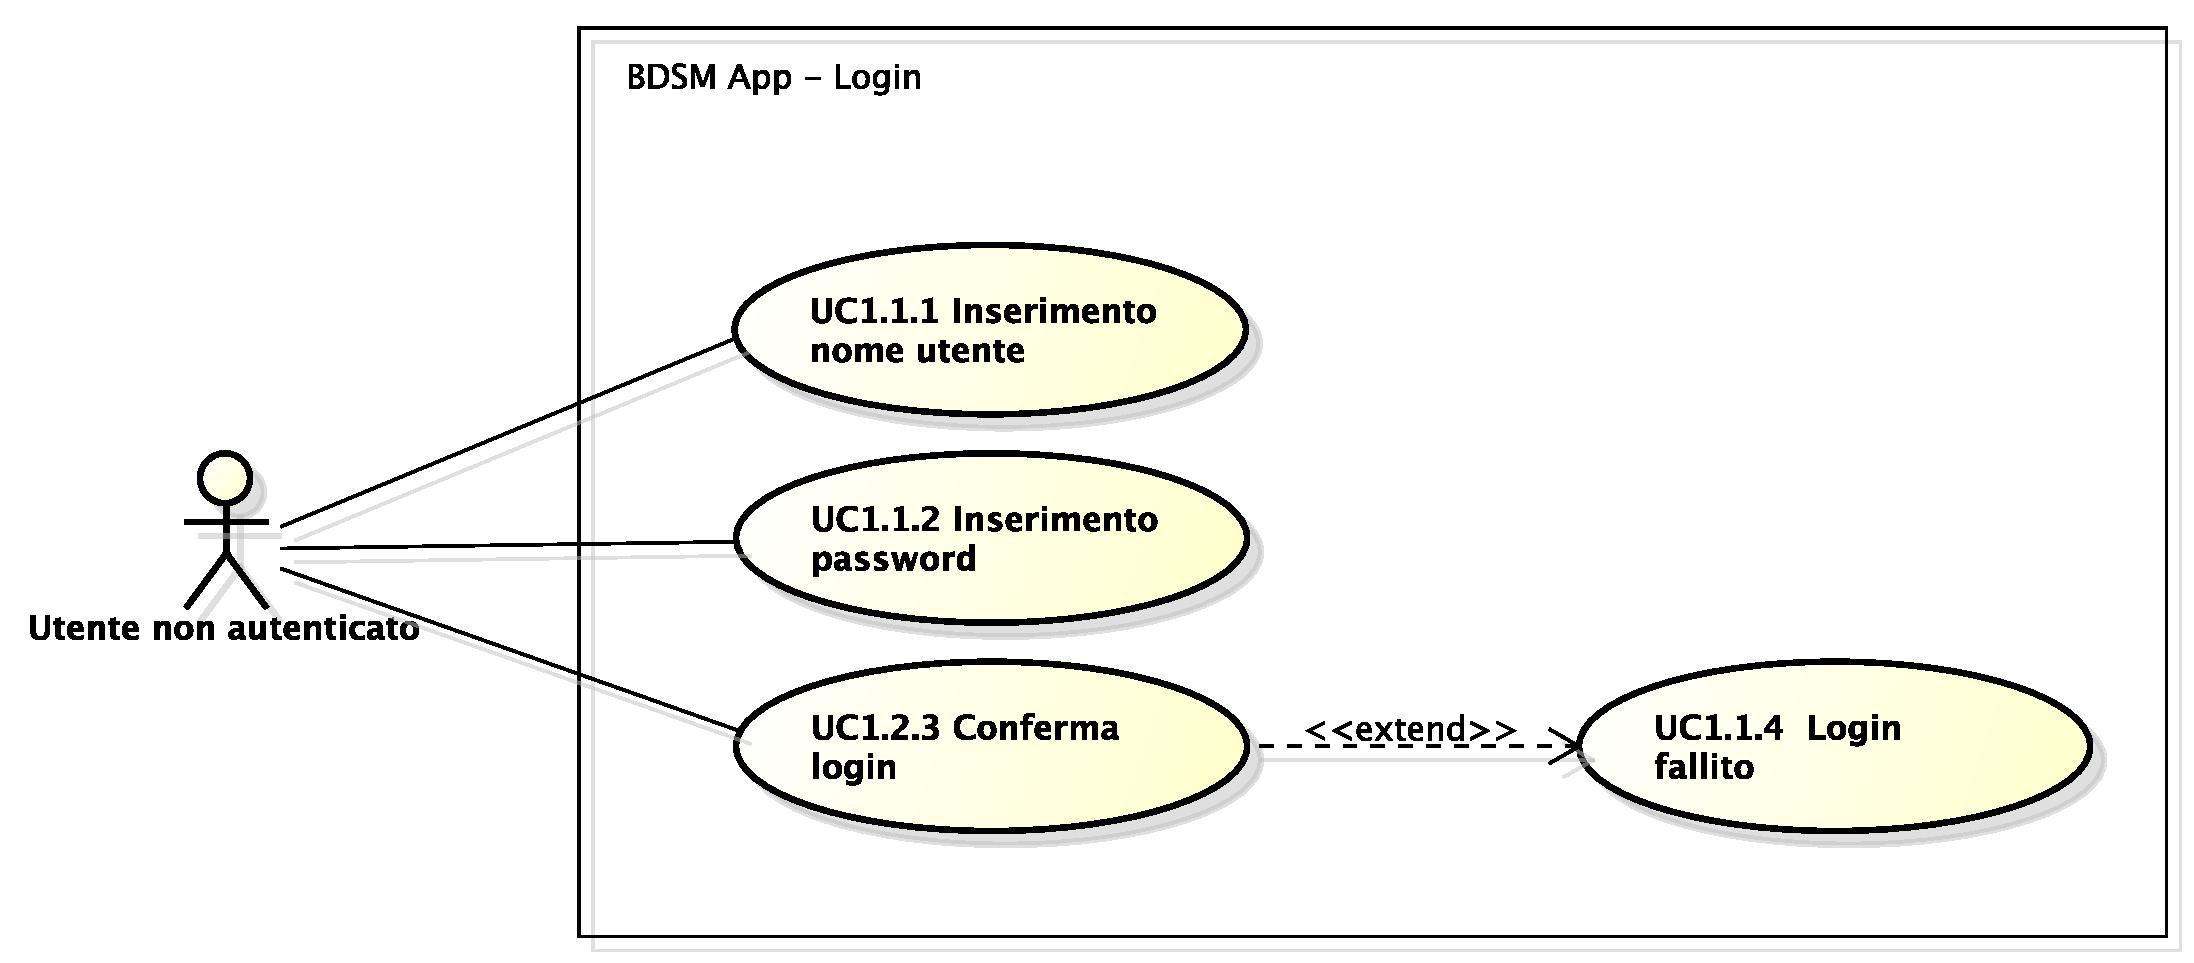
\includegraphics[scale=0.45]{./images/UC1_1.pdf}}
			\caption{D3.3 - Diagramma dell'amministrazione degli utenti}
		\end{figure}
		[TO DO] (descrizione generale)
		% subsubsection amministrazione_degli_utenti (end)




	% subsection utente_amministratore (end)




% section diagrammi_delle_attività (end) \clearpage \newpage
% =================================================================================================
% File:			design_pattern.tex
% Description:	Defiinisce la sezione relativa a ...
% Created:		2015-02-23
% Author:		Tesser Paolo
% Email:		tesser.paolo@mashup-unipd.it
% =================================================================================================
% Modification History:
% Version		Modifier Date		Change											Author
% 0.0.1 		2015-02-23 			sistemato header								Tesser Paolo
% =================================================================================================
% 0.0.2			2015-03-31			aggiunta introduzione ai DP						Tesser Paolo
% =================================================================================================
%


% CONTENUTO DEL CAPITOLO

\section{Design Pattern} % (fold)
\label{sec:design_pattern}
In questa sezione verranno presentati i diversi design pattern utilizzati per la progettazione architetturale. I design pattern sono soluzioni a problemi ricorrenti. Adottarli porta diversi benefici:
	\begin{itemize}
		\item favorisce il riutilizzo del codice;
		\item semplifica l’attività di progettazione;
		\item rende l’architettura più manutenibile.
	\end{itemize}
	\noindent
I design pattern possono essere suddivisi in:
	\begin{itemize}
		\item \textbf{Architetturali}: definiscono l’architettura dell’applicazione ad un livello elevato;
		\item \textbf{Creazionali}: permettono di nascondere i costruttori delle classi, consentendo la creazione di oggetti senza conoscerne la loro implementazione;
		\item \textbf{Strutturali}: consentono di riutilizzare classi preesistenti, fornendo un’interfaccia più adatta;
		\item \textbf{Comportamentali}: definiscono soluzioni per le interazioni tra oggetti.
	\end{itemize}
	\noindent
	\newline
Per una descrizione più approfondita dei design pattern utilizzati si faccia riferimento all’appendice \ref{sec:descdp}. I vari diagrammi che riprendono l’architettura non espongono tutte le sottoclassi e i metodi delle stesse. Lo scopo dei diagrammi è di mostrare le caratteristiche del design pattern adottato e come le varie classi interagiscono tra di loro. Nella realizzazione del progetto \projectName{} si è deciso di implementare i seguenti design pattern.

	\pagebreak

	% =================================================================================================
% File:			dp_architetturali.tex
% Description:	Defiinisce la sezione relativa a ...
% Created:		2015-03-26
% Author:		Tesser Paolo
% Email:		tesser.paolo@mashup-unipd.it
% =================================================================================================
% Modification History:
% Version		Modifier Date		Change											Author
% 0.0.1 		2015-03-26 			aggiunto sezioni								Tesser Paolo
% =================================================================================================
% 0.0.2			2015-04-03			descritto pattern MVC, MVW e DI					Tesser Paolo
% =================================================================================================
% 0.0.3			2015-04-13			descritto Three-Tier							Tesser Paolo
% =================================================================================================
%

% CONTENUTO DEL CAPITOLO

\subsection{Design pattern architetturali} % (fold)
\label{sub:design_pattern_architetturali}
	\subsubsection{Three-Tier} % (fold)
	\label{ssub:three_tier}
		\begin{itemize}
			\item \textbf{Scope dell'utilizzo}: è stato scelto il pattern Three-tier per rendere massima la distribuzione delle componenti principali del sistema: client(front-end), server(back-end) e database (Datastore). La decisione di adottare un'architettura REST-like ha contribuito alla scelta dell'infrastruttura, che ci permette di separare al meglio le diverse parti;
			\item \textbf{Contesto dell'utilizzo}:
				\begin{itemize}
					\item \textbf{Intera applicazione}: la decomposizione del sistema avviene secondo lo schema citato precedentemente. Ogni componente rappresenta un livello del pattern. Il client comunica con il server attraverso i servizi REST esposti da quest'ultimo, mentre il server comunica con il database attraverso le funzionalità offerte dalla Google App Engine. \newline
					[TO DO] (grafico del pattern applicato al caso di utilizzo nell'applicativo)
				\end{itemize}
		\end{itemize}
	% subsubsection three_tier (end)


	\subsubsection{MVW} % (fold)
	\label{ssub:mvw}
		\begin{itemize}
			\item \textbf{Scope dell'utilizzo}: è un Design Pattern simile a MVC, che permette di avere una corrispondenza più diretta e automatica tra la \emph{view} e il \emph{model}. L'acronimo MVW sta infatti per Model-View-Whatever, dove \emph{Whatever} indica \emph{``whatever works for you''};
			\item \textbf{Contesto dell'utilizzo}: 
				\begin{itemize}
					\item \textbf{Client}: viene utilizzato per gestire il lato client dell'applicazione. Questo ci viene fornito direttamente dal framework AngularJS. La parte W (Whatever) assume internamente due diversi aspetti. \newline
					Il diagramma che riporta lo schema del pattern è quello presente alla sezione \ref{sub:client}.
				\end{itemize}
		\end{itemize}

		\paragraph{MVC} % (fold)
		\label{par:mvc}
			\begin{itemize}
				\item \textbf{Scope dell'utilizzo}: questo pattern è utilizzato per separare le responsabilità dell’applicazione a diversi componenti e permettere di fare una chiara divisione tra presentazione, struttura dei dati e operazioni su di essi;

				\item \textbf{Contesto dell'utilizzo}: 
					\begin{itemize}
						\item \textbf{Client}: viene utilizzato nel livello client per separare i componenti a seconda delle loro responsabilità e secondo una connotazione semantica. Il formalismo che viene quindi assunto per dividere i package è proprio quello fornito dal pattern in questione e cioè: \textbf{model, view e controller}. Questi però non interagiscono tra di loro nella maniera canonica che il pattern offre, ma seguono lo stile proposto da MVVM descritto alla sezione \ref{par:mvvm}.
					\end{itemize}
			\end{itemize}
		% paragraph mvc (end)

		\paragraph{MVVM} % (fold)
		\label{par:mvvm}
			\begin{itemize}
				\item \textbf{Scope dell'utilizzo}: questo pattern è utilizzato per gestire il modo con il quale le diverse parti comunicano tra loro per scambiare i dati e per gestire le operazioni che l'utente richiede attraverso l'interazione con la View;

				\item \textbf{Contesto dell'utilizzo}: 
					\begin{itemize}
						\item \textbf{Client}: viene utilizzato nel livello client per gestire lo scambio dei dati e le interazioni che fanno cambiare le View e lo stato del Model, attraverso principalmente un sistema di two-way data binding e di eventi. Il Model però non interagisce direttamente con le View, ma passa attraverso un controller che fa da collante tra la View e il Model (ViewModel) attraverso l'oggetto \$scope.
					\end{itemize}
			\end{itemize}
		% paragraph mvvm (end)
	% subsubsection mvw (end)

	\subsubsection{Dependency Injection} % (fold)
	\label{ssub:dependency_injection}
		\begin{itemize}
			\item \textbf{Scope dell'utilizzo}: è un Design Pattern che viene utilizzato per favorire la separazione delle responsabilità tra i componenti dalla risoluzione delle dipendenze. Questo permette di avere una migliore modularità del codice, di avere un minor accoppiamento tra le diverse parti e garantisce una più facile fase di testing;
			\item \textbf{Contesto dell'utilizzo}: 
				\begin{itemize}
					\item \textbf{Client}: viene utilizzato direttamente da AngularJS per iniettare le diverse dipendenze nei moduli che le richiedono. In particolare vengono iniettati nei controller tutti i servizi e i modelli dei dati necessari all'interazione dell'utente con le viste. \newline
					Non ne viene fornita nessuna rappresentazione grafica in quanto non è una cosa che viene progettata dal team, ma usata direttamente attraverso il framework scelto;
				\end{itemize}
		\end{itemize}
	% subsubsection dependency_injection (end)

% subsection design_pattern_architetturali (end) \clearpage \newpage
	% =================================================================================================
% File:			dp_creazionali.tex
% Description:	Defiinisce la sezione relativa a ...
% Created:		2015-03-26
% Author:		Tesser Paolo
% Email:		tesser.paolo@mashup-unipd.it
% =================================================================================================
% Modification History:
% Version		Modifier Date		Change											Author
% 0.0.1 		2015-03-26 			creato scheltro sezione							Tesser Paolo
% =================================================================================================
% 0.0.2			2015-04-08			inserito scheletro per DP: Prototype e Module	Tesser Paolo
% =================================================================================================
%

% CONTENUTO DEL CAPITOLO

\subsection{Design pattern creazionali} % (fold)
\label{sub:design_pattern_creazionali}
	\subsubsection{Prototype Pattern} % (fold)
	\label{ssub:prototype_pattern}
	[TO DO] (grafico del pattern applicato al caso di utilizzo nell'applicativo)
		\begin{itemize}
			\item \textbf{Scope dell'utilizzo}: [TO DO];
			\item \textbf{Contesto dell'utilizzo}: [TO DO];
		\end{itemize}
	% subsubsection prototype_pattern (end)

	\subsubsection{Module Pattern} % (fold)
	\label{ssub:module_pattern}
	[TO DO] (grafico del pattern applicato al caso di utilizzo nell'applicativo)
		\begin{itemize}
			\item \textbf{Scope dell'utilizzo}: [TO DO];
			\item \textbf{Contesto dell'utilizzo}: [TO DO];
		\end{itemize}
	% subsubsection module_pattern (end)
% subsection design_pattern_creazionali (end) \clearpage \newpage
	% =================================================================================================
% File:			dp_strutturali.tex
% Description:	Defiinisce la sezione relativa a ...
% Created:		2015-03-26
% Author:		Tesser Paolo
% Email:		tesser.paolo@mashup-unipd.it
% =================================================================================================
% Modification History:
% Version		Modifier Date		Change											Author
% 0.0.1 		2015-03-26 			sistemato header								Tesser Paolo
% =================================================================================================
% 0.0.2			2015-04-08			aggiunto scheletro per pattern Facade			Tesser Paolo
% =================================================================================================
%

% CONTENUTO DEL CAPITOLO

\subsection{Design pattern strutturali} % (fold)
\label{sub:design_pattern_strutturali}
	\subsubsection{Fa\c{c}ade} % (fold)
	\label{ssub:facade}
	[TO DO] (grafico del pattern applicato al caso di utilizzo nell'applicativo)
		\begin{itemize}
			\item \textbf{Scope dell'utilizzo}: [TO DO];
			\item \textbf{Contesto dell'utilizzo}: [TO DO];
		\end{itemize}
	% subsubsection facade (end)



% subsection design_pattern_strutturali (end) \clearpage \newpage
	% =================================================================================================
% File:			dp_comportamentali.tex
% Description:	Defiinisce la sezione relativa a ...
% Created:		2015-03-26
% Author:		Tesser Paolo
% Email:		tesser.paolo@mashup-unipd.it
% =================================================================================================
% Modification History:
% Version		Modifier Date		Change											Author
% 0.0.1 		2015-03-26 			sistemato header								Tesser Paolo
% =================================================================================================
% 0.0.2			2015-04-14			descritit DP Page Controller, Template View		Tesser Paolo
% =================================================================================================
% 0.0.3			2015-04-14			descritto DP Template Method					Tesser Paolo
% =================================================================================================
%

% CONTENUTO DEL CAPITOLO

\subsection{Design pattern comportamentali} % (fold)
\label{sub:design_pattern_comportamentali}
	\subsubsection{Page Controller} % (fold)
	\label{ssub:page_controller}
		\begin{itemize}
			\item \textbf{Scope dell'utilizzo}: questo pattern serve [TO DO];
			\item \textbf{Contesto dell'utilizzo}:
				\begin{itemize}
					\item \textbf{Client}: viene utilizzato \newline
					[TO DO] (grafico del pattern applicato al caso di utilizzo nell'applicativo)
				\end{itemize}
		\end{itemize}
	% subsubsection page_controller (end)


	\subsubsection{Template Method} % (fold)
	\label{ssub:template_method}
		\begin{itemize}
			\item \textbf{Scope dell'utilizzo}: questo pattern serve per definire lo scheletro di un algoritmo, lasciando l'implementazione di alcuni passi alle sottoclassi;
			\item \textbf{Contesto dell'utilizzo}:
				\begin{itemize}
					\item \textbf{Client}: viene utilizzato nel package \ref{ssub:bdsm_app_client_model_services}, per permettere di generare tipi di grafici diversi che però hanno in comune la prima parte dell'algoritmo che li genera. In particolare la parte comune si occupa del recupero dei dati a prescindere da quali grafico li userà. [TO DO] \newline
					[TO DO] (grafico del pattern applicato al caso di utilizzo nell'applicativo)

					\item \textbf{Server}: [TO DO]. \newline
					[TO DO] (grafico del pattern applicato al caso di utilizzo nell'applicativo)
				\end{itemize}
		\end{itemize}
	% subsubsection template_method (end)


	\subsubsection{Template View} % (fold)
	\label{ssub:template_view}
		\begin{itemize}
			\item \textbf{Scope dell'utilizzo}: questo pattern serve per interpretare alcune informazioni incorporate nei template HTML. Nei sistemi di template generalmente vengono utilizzati dei segnaposto (markers) di qualche formato che verranno interpretati e sostituiti con il codice HTML adeguato. In AngularJS invece non c'è un formato intermediario perché vengono usate direttamente delle direttive HTML che quando saranno trovate dal compilatore di Angular, verrà invocata la logica ad esse associata;
			\item \textbf{Contesto dell'utilizzo}:
				\begin{itemize}
					\item \textbf{Client}: viene utilizzato in tutti i template HTML presentati nel package \textt{client::view} presente alla sezione \ref{ssub:bdsm_app_client_view}. \newline
					Ne viene qui di seguito illustrata una implementazione relativa al template HTML Settings. \newline
					[TO DO]
				\end{itemize}
		\end{itemize}
	% subsubsection template_view (end)


	\subsubsection{Command} % (fold)
	\label{ssub:command}
	[TO DO] (grafico del pattern applicato al caso di utilizzo nell'applicativo)
		\begin{itemize}
			\item \textbf{Scope dell'utilizzo}: [TO DO];
			\item \textbf{Contesto dell'utilizzo}:
				\begin{itemize}
					\item \textbf{Server}: [TO DO]
				\end{itemize}
		\end{itemize}
	% subsubsection command (end)
% subsection design_pattern_comportamentali (end) \clearpage \newpage
% section design_pattern (end)
 \clearpage \newpage
% =================================================================================================
% File:			stime_fattibilita.tex
% Description:	Defiinisce la sezione relativa a ...
% Created:		2015-02-23
% Author:		Tesser Paolo
% Email:		tesser.paolo@mashup-unipd.it
% =================================================================================================
% Modification History:
% Version		Modifier Date		Change											Author
% 0.0.1 		2015-02-23 			sistemato header								Tesser Paolo
% =================================================================================================
%
% =================================================================================================
%

% CONTENUTO DEL CAPITOLO

\section{Stime di fattibilità} % (fold)
\label{sec:stime_di_fattibilita}

% section stime_di_fattibilità (end) \clearpage \newpage
% =================================================================================================
% File:			capitolo_3.tex
% Description:	Definisce il capitolo che descrive generalmente il prodotto per il commitente
% Created:		2014/12/10
% Author:		Roetta Marco
% Email:		roetta.marco@mashup-unipd.it
% =================================================================================================
% Modification History:
% Version		Modifier Date		Change											Author
% 0.0.1 		2014/12/10 			aggiunta sezione e iniziata stesura				Roetta Marco
% =================================================================================================
%

% CONTENUTO DEL CAPITOLO

\section{Tracciamento requisiti-test}
In questa sezione vengono riportati, per ogni requisito, il corrispondente test di
sistema e test di validazione. I requisiti di qualità non sono tracciati in quanto sono verificati
costantemente durante tutto lo sviluppo del progetto.




 \clearpage \newpage
% da mettere come appendice e non rientrante nella numerazione standard dell'indice
% =================================================================================================
% File:			mockup.tex
% Description:	Defiinisce la sezione relativa al bmockup dell'applicazione web
% Created:		2015-03-27
% Author:		Tesser Paolo
% Email:		tesser.paolo@mashup-unipd.it
% =================================================================================================
% Modification History:
% Version		Modifier Date		Change											Author
% 0.0.1 		2015-03-27 			creato scheletro								Tesser Paolo
% =================================================================================================
%
% =================================================================================================
%

% CONTENUTO DEL CAPITOLO
\appendix


\section{Mockup} % (fold)
\label{sec:mockup}
	\subsection{Login} % (fold)
	\label{sub:login}
		\subsubsection{Descrizione generale} % (fold)
		[TO DO]
		% subsubsection descrizione_generale (end)

		\subsubsection{Vista desktop} % (fold)
		[TO DO] (inserire immagine)
		% subsubsection vista_desktop (end)

		\subsubsection{Vista mobile} % (fold)
		[TO DO] (inserire immagine)
		% subsubsection vista_mobile (end)
	% subsection login (end)

	\subsection{Register} % (fold)
	\label{sub:register}
		\subsubsection{Descrizione generale} % (fold)
		[TO DO]
		% subsubsection descrizione_generale (end)

		\subsubsection{Vista desktop} % (fold)
		[TO DO] (inserire immagine)
		% subsubsection vista_desktop (end)

		\subsubsection{Vista mobile} % (fold)
		[TO DO] (inserire immagine)
		% subsubsection vista_mobile (end)
	% subsection register (end)

	\subsection{Recipe} % (fold)
	\label{sub:recipe}
		\subsubsection{Descrizione generale} % (fold)
		[TO DO]
		% subsubsection descrizione_generale (end)

		\subsubsection{Vista desktop} % (fold)
		[TO DO] (inserire immagine)
		% subsubsection vista_desktop (end)

		\subsubsection{Vista mobile} % (fold)
		[TO DO] (inserire immagine)
		% subsubsection vista_mobile (end)
	% subsection recipe (end)

	\subsection{Metrics} % (fold)
	\label{sub:metrics}
		\subsubsection{Descrizione generale} % (fold)
		[TO DO]
		% subsubsection descrizione_generale (end)

		\subsubsection{Vista desktop} % (fold)
		[TO DO] (inserire immagine)
		% subsubsection vista_desktop (end)

		\subsubsection{Vista mobile} % (fold)
		[TO DO] (inserire immagine)
		% subsubsection vista_mobile (end)
	% subsubsection metrics (end)

	\subsection{Settings} % (fold)
	\label{sub:settings}
		\subsubsection{Descrizione generale} % (fold)
		[TO DO]
		% subsubsection descrizione_generale (end)

		\subsubsection{Vista desktop} % (fold)
		[TO DO] (inserire immagine)
		% subsubsection vista_desktop (end)

		\subsubsection{Vista mobile} % (fold)
		[TO DO] (inserire immagine)
		% subsubsection vista_mobile (end)
	% subsection settings (end)

	\subsection{Insert} % (fold)
	\label{sub:insert}
		\subsubsection{Descrizione generale} % (fold)
		[TO DO]
		% subsubsection descrizione_generale (end)

		\subsubsection{Vista desktop} % (fold)
		[TO DO] (inserire immagine)
		% subsubsection vista_desktop (end)

		\subsubsection{Vista mobile} % (fold)
		[TO DO] (inserire immagine)
		% subsubsection vista_mobile (end)
	% subsubsection insert (end)






	\subsection{Pagina} % (fold)
	\label{sub:pagina}
		\subsubsection{Descrizione generale} % (fold)
		[TO DO]
		% subsubsection descrizione_generale (end)

		\subsubsection{Vista desktop} % (fold)
		[TO DO] (inserire immagine)
		% subsubsection vista_desktop (end)

		\subsubsection{Vista mobile} % (fold)
		[TO DO] (inserire immagine)
		% subsubsection vista_mobile (end)
	% subsection pagina (end)
% section mockup (end) \clearpage \newpage